
%% bare_jrnl.tex
%% V1.4b
%% 2015/08/26
%% by Michael Shell
%% see http://www.michaelshell.org/
%% for current contact information.
%%
%% This is a skeleton file demonstrating the use of IEEEtran.cls
%% (requires IEEEtran.cls version 1.8b or later) with an IEEE
%% journal paper.
%%
%% Support sites:
%% http://www.michaelshell.org/tex/ieeetran/
%% http://www.ctan.org/pkg/ieeetran
%% and
%% http://www.ieee.org/

%%*************************************************************************
%% Legal Notice:
%% This code is offered as-is without any warranty either expressed or
%% implied; without even the implied warranty of MERCHANTABILITY or
%% FITNESS FOR A PARTICULAR PURPOSE! 
%% User assumes all risk.
%% In no event shall the IEEE or any contributor to this code be liable for
%% any damages or losses, including, but not limited to, incidental,
%% consequential, or any other damages, resulting from the use or misuse
%% of any information contained here.
%%
%% All comments are the opinions of their respective authors and are not
%% necessarily endorsed by the IEEE.
%%
%% This work is distributed under the LaTeX Project Public License (LPPL)
%% ( http://www.latex-project.org/ ) version 1.3, and may be freely used,
%% distributed and modified. A copy of the LPPL, version 1.3, is included
%% in the base LaTeX documentation of all distributions of LaTeX released
%% 2003/12/01 or later.
%% Retain all contribution notices and credits.
%% ** Modified files should be clearly indicated as such, including  **
%% ** renaming them and changing author support contact information. **
%%*************************************************************************


% *** Authors should verify (and, if needed, correct) their LaTeX system  ***
% *** with the testflow diagnostic prior to trusting their LaTeX platform ***
% *** with production work. The IEEE's font choices and paper sizes can   ***
% *** trigger bugs that do not appear when using other class files.       ***                          ***
% The testflow support page is at:
% http://www.michaelshell.org/tex/testflow/



\documentclass[journal]{IEEEtran}
%
% If IEEEtran.cls has not been installed into the LaTeX system files,
% manually specify the path to it like:
% \documentclass[journal]{../sty/IEEEtran}





% Some very useful LaTeX packages include:
% (uncomment the ones you want to load)


% *** MISC UTILITY PACKAGES ***
%
%\usepackage{ifpdf}
% Heiko Oberdiek's ifpdf.sty is very useful if you need conditional
% compilation based on whether the output is pdf or dvi.
% usage:
% \ifpdf
%   % pdf code
% \else
%   % dvi code
% \fi
% The latest version of ifpdf.sty can be obtained from:
% http://www.ctan.org/pkg/ifpdf
% Also, note that IEEEtran.cls V1.7 and later provides a builtin
% \ifCLASSINFOpdf conditional that works the same way.
% When switching from latex to pdflatex and vice-versa, the compiler may
% have to be run twice to clear warning/error messages.






% *** CITATION PACKAGES ***
%
\usepackage{cite}
% cite.sty was written by Donald Arseneau
% V1.6 and later of IEEEtran pre-defines the format of the cite.sty package
% \cite{} output to follow that of the IEEE. Loading the cite package will
% result in citation numbers being automatically sorted and properly
% "compressed/ranged". e.g., [1], [9], [2], [7], [5], [6] without using
% cite.sty will become [1], [2], [5]--[7], [9] using cite.sty. cite.sty's
% \cite will automatically add leading space, if needed. Use cite.sty's
% noadjust option (cite.sty V3.8 and later) if you want to turn this off
% such as if a citation ever needs to be enclosed in parenthesis.
% cite.sty is already installed on most LaTeX systems. Be sure and use
% version 5.0 (2009-03-20) and later if using hyperref.sty.
% The latest version can be obtained at:
% http://www.ctan.org/pkg/cite
% The documentation is contained in the cite.sty file itself.






% *** GRAPHICS RELATED PACKAGES ***
\usepackage{graphicx}
\graphicspath{ {./images/} }
%
%\ifCLASSINFOpdf
  %\usepackage[pdftex]{graphicx}
  % declare the path(s) where your graphic files are
  % \graphicspath{{../pdf/}{../jpeg/}}
  % and their extensions so you won't have to specify these with
  % every instance of \includegraphics
%  \DeclareGraphicsExtensions{.png}
%\else
  % or other class option (dvipsone, dvipdf, if not using dvips). graphicx
  % will default to the driver specified in the system graphics.cfg if no
  % driver is specified.
  % \usepackage[dvips]{graphicx}
  % declare the path(s) where your graphic files are
  % \graphicspath{{../eps/}}
  % and their extensions so you won't have to specify these with
  % every instance of \includegraphics
  % \DeclareGraphicsExtensions{.eps}
%\fi
% graphicx was written by David Carlisle and Sebastian Rahtz. It is
% required if you want graphics, photos, etc. graphicx.sty is already
% installed on most LaTeX systems. The latest version and documentation
% can be obtained at: 
% http://www.ctan.org/pkg/graphicx
% Another good source of documentation is "Using Imported Graphics in
% LaTeX2e" by Keith Reckdahl which can be found at:
% http://www.ctan.org/pkg/epslatex
%
% latex, and pdflatex in dvi mode, support graphics in encapsulated
% postscript (.eps) format. pdflatex in pdf mode supports graphics
% in .pdf, .jpeg, .png and .mps (metapost) formats. Users should ensure
% that all non-photo figures use a vector format (.eps, .pdf, .mps) and
% not a bitmapped formats (.jpeg, .png). The IEEE frowns on bitmapped formats
% which can result in "jaggedy"/blurry rendering of lines and letters as
% well as large increases in file sizes.
%
% You can find documentation about the pdfTeX application at:
% http://www.tug.org/applications/pdftex





% *** MATH PACKAGES ***
%
\usepackage{amsmath}
% A popular package from the American Mathematical Society that provides
% many useful and powerful commands for dealing with mathematics.
%
% Note that the amsmath package sets \interdisplaylinepenalty to 10000
% thus preventing page breaks from occurring within multiline equations. Use:
%\interdisplaylinepenalty=2500
% after loading amsmath to restore such page breaks as IEEEtran.cls normally
% does. amsmath.sty is already installed on most LaTeX systems. The latest
% version and documentation can be obtained at:
% http://www.ctan.org/pkg/amsmath





% *** SPECIALIZED LIST PACKAGES ***
%
\usepackage{algorithm,algorithmic}
% algorithmic.sty was written by Peter Williams and Rogerio Brito.
% This package provides an algorithmic environment fo describing algorithms.
% You can use the algorithmic environment in-text or within a figure
% environment to provide for a floating algorithm. Do NOT use the algorithm
% floating environment provided by algorithm.sty (by the same authors) or
% algorithm2e.sty (by Christophe Fiorio) as the IEEE does not use dedicated
% algorithm float types and packages that provide these will not provide
% correct IEEE style captions. The latest version and documentation of
% algorithmic.sty can be obtained at:
% http://www.ctan.org/pkg/algorithms
% Also of interest may be the (relatively newer and more customizable)
% algorithmicx.sty package by Szasz Janos:
% http://www.ctan.org/pkg/algorithmicx




% *** ALIGNMENT PACKAGES ***
%
\usepackage{array}
% Frank Mittelbach's and David Carlisle's array.sty patches and improves
% the standard LaTeX2e array and tabular environments to provide better
% appearance and additional user controls. As the default LaTeX2e table
% generation code is lacking to the point of almost being broken with
% respect to the quality of the end results, all users are strongly
% advised to use an enhanced (at the very least that provided by array.sty)
% set of table tools. array.sty is already installed on most systems. The
% latest version and documentation can be obtained at:
% http://www.ctan.org/pkg/array


% IEEEtran contains the IEEEeqnarray family of commands that can be used to
% generate multiline equations as well as matrices, tables, etc., of high
% quality.




% *** SUBFIGURE PACKAGES ***
%\ifCLASSOPTIONcompsoc
%  \usepackage[caption=false,font=normalsize,labelfont=sf,textfont=sf]{subfig}
%\else
  \usepackage[caption=false,font=footnotesize]{subfig}
%\fi
% subfig.sty, written by Steven Douglas Cochran, is the modern replacement
% for subfigure.sty, the latter of which is no longer maintained and is
% incompatible with some LaTeX packages including fixltx2e. However,
% subfig.sty requires and automatically loads Axel Sommerfeldt's caption.sty
% which will override IEEEtran.cls' handling of captions and this will result
% in non-IEEE style figure/table captions. To prevent this problem, be sure
% and invoke subfig.sty's "caption=false" package option (available since
% subfig.sty version 1.3, 2005/06/28) as this is will preserve IEEEtran.cls
% handling of captions.
% Note that the Computer Society format requires a larger sans serif font
% than the serif footnote size font used in traditional IEEE formatting
% and thus the need to invoke different subfig.sty package options depending
% on whether compsoc mode has been enabled.
%
% The latest version and documentation of subfig.sty can be obtained at:
% http://www.ctan.org/pkg/subfig




% *** FLOAT PACKAGES ***
%
%\usepackage{fixltx2e}
% fixltx2e, the successor to the earlier fix2col.sty, was written by
% Frank Mittelbach and David Carlisle. This package corrects a few problems
% in the LaTeX2e kernel, the most notable of which is that in current
% LaTeX2e releases, the ordering of single and double column floats is not
% guaranteed to be preserved. Thus, an unpatched LaTeX2e can allow a
% single column figure to be placed prior to an earlier double column
% figure.
% Be aware that LaTeX2e kernels dated 2015 and later have fixltx2e.sty's
% corrections already built into the system in which case a warning will
% be issued if an attempt is made to load fixltx2e.sty as it is no longer
% needed.
% The latest version and documentation can be found at:
% http://www.ctan.org/pkg/fixltx2e


%\usepackage{stfloats}
% stfloats.sty was written by Sigitas Tolusis. This package gives LaTeX2e
% the ability to do double column floats at the bottom of the page as well
% as the top. (e.g., "\begin{figure*}[!b]" is not normally possible in
% LaTeX2e). It also provides a command:
%\fnbelowfloat
% to enable the placement of footnotes below bottom floats (the standard
% LaTeX2e kernel puts them above bottom floats). This is an invasive package
% which rewrites many portions of the LaTeX2e float routines. It may not work
% with other packages that modify the LaTeX2e float routines. The latest
% version and documentation can be obtained at:
% http://www.ctan.org/pkg/stfloats
% Do not use the stfloats baselinefloat ability as the IEEE does not allow
% \baselineskip to stretch. Authors submitting work to the IEEE should note
% that the IEEE rarely uses double column equations and that authors should try
% to avoid such use. Do not be tempted to use the cuted.sty or midfloat.sty
% packages (also by Sigitas Tolusis) as the IEEE does not format its papers in
% such ways.
% Do not attempt to use stfloats with fixltx2e as they are incompatible.
% Instead, use Morten Hogholm'a dblfloatfix which combines the features
% of both fixltx2e and stfloats:
%
% \usepackage{dblfloatfix}
% The latest version can be found at:
% http://www.ctan.org/pkg/dblfloatfix




%\ifCLASSOPTIONcaptionsoff
%  \usepackage[nomarkers]{endfloat}
% \let\MYoriglatexcaption\caption
% \renewcommand{\caption}[2][\relax]{\MYoriglatexcaption[#2]{#2}}
%\fi
% endfloat.sty was written by James Darrell McCauley, Jeff Goldberg and 
% Axel Sommerfeldt. This package may be useful when used in conjunction with 
% IEEEtran.cls'  captionsoff option. Some IEEE journals/societies require that
% submissions have lists of figures/tables at the end of the paper and that
% figures/tables without any captions are placed on a page by themselves at
% the end of the document. If needed, the draftcls IEEEtran class option or
% \CLASSINPUTbaselinestretch interface can be used to increase the line
% spacing as well. Be sure and use the nomarkers option of endfloat to
% prevent endfloat from "marking" where the figures would have been placed
% in the text. The two hack lines of code above are a slight modification of
% that suggested by in the endfloat docs (section 8.4.1) to ensure that
% the full captions always appear in the list of figures/tables - even if
% the user used the short optional argument of \caption[]{}.
% IEEE papers do not typically make use of \caption[]'s optional argument,
% so this should not be an issue. A similar trick can be used to disable
% captions of packages such as subfig.sty that lack options to turn off
% the subcaptions:
% For subfig.sty:
% \let\MYorigsubfloat\subfloat
% \renewcommand{\subfloat}[2][\relax]{\MYorigsubfloat[]{#2}}
% However, the above trick will not work if both optional arguments of
% the \subfloat command are used. Furthermore, there needs to be a
% description of each subfigure *somewhere* and endfloat does not add
% subfigure captions to its list of figures. Thus, the best approach is to
% avoid the use of subfigure captions (many IEEE journals avoid them anyway)
% and instead reference/explain all the subfigures within the main caption.
% The latest version of endfloat.sty and its documentation can obtained at:
% http://www.ctan.org/pkg/endfloat
%
% The IEEEtran \ifCLASSOPTIONcaptionsoff conditional can also be used
% later in the document, say, to conditionally put the References on a 
% page by themselves.




% *** PDF, URL AND HYPERLINK PACKAGES ***
%
\usepackage{url}
% url.sty was written by Donald Arseneau. It provides better support for
% handling and breaking URLs. url.sty is already installed on most LaTeX
% systems. The latest version and documentation can be obtained at:
% http://www.ctan.org/pkg/url
% Basically, \url{my_url_here}.




% *** Do not adjust lengths that control margins, column widths, etc. ***
% *** Do not use packages that alter fonts (such as pslatex).         ***
% There should be no need to do such things with IEEEtran.cls V1.6 and later.
% (Unless specifically asked to do so by the journal or conference you plan
% to submit to, of course. )

%Alessandro input: makecell package to permite line break inside tables
\usepackage{makecell}
\usepackage{xcolor}

% correct bad hyphenation here
\hyphenation{op-tical net-works semi-conduc-tor}

\renewcommand{\baselinestretch}{0.96}

\begin{document}
%
% paper title
% Titles are generally capitalized except for words such as a, an, and, as,
% at, but, by, for, in, nor, of, on, or, the, to and up, which are usually
% not capitalized unless they are the first or last word of the title.
% Linebreaks \\ can be used within to get better formatting as desired.
% Do not put math or special symbols in the title.
%\title{Building a framework to perform automated verification of solar photovoltaic off-grid systems}
\title{Automated Verification of Stand-Alone Solar Photovoltaic Systems}
%
%
% author names and IEEE memberships
% note positions of commas and nonbreaking spaces ( ~ ) LaTeX will not break
% a structure at a ~ so this keeps an author's name from being broken across
% two lines.
% use \thanks{} to gain access to the first footnote area
% a separate \thanks must be used for each paragraph as LaTeX2e's \thanks
% was not built to handle multiple paragraphs
%

\author{Alessandro~Trindade and Lucas~Cordeiro% <-this % stops a space
\thanks{A. Trindade is with the Department of Electricity, Federal University of Amazonas, Manaus, Brazil, e-mail: alessandrotrindade@ufam.edu.br.}% <-this % stops a space
\thanks{L. Cordeiro is with School of Computer Science, The University of Manchester, UK, e-mail: lucas.cordeiro@manchester.ac.uk.}% <-this % stops a space
\thanks{The authors would like to thank Newton Fund (ref. 261881580) and FAPEAM (Amazonas State Foundation for Research Support, call 009/2017), for the financial support.}
\thanks{Manuscript received November 23, 2018; revised XXXXX 11, 2019.}}

% note the % following the last \IEEEmembership and also \thanks - 
% these prevent an unwanted space from occurring between the last author name
% and the end of the author line. i.e., if you had this:
% 
% \author{....lastname \thanks{...} \thanks{...} }
%                     ^------------^------------^----Do not want these spaces!
%
% a space would be appended to the last name and could cause every name on that
% line to be shifted left slightly. This is one of those "LaTeX things". For
% instance, "\textbf{A} \textbf{B}" will typeset as "A B" not "AB". To get
% "AB" then you have to do: "\textbf{A}\textbf{B}"
% \thanks is no different in this regard, so shield the last } of each \thanks
% that ends a line with a % and do not let a space in before the next \thanks.
% Spaces after \IEEEmembership other than the last one are OK (and needed) as
% you are supposed to have spaces between the names. For what it is worth,
% this is a minor point as most people would not even notice if the said evil
% space somehow managed to creep in.



% The paper headers
\markboth{IEEE TRANSACTIONS ON SUSTAINABLE ENERGY,~VOL.~X, NO.~Y, MONTH~2018}
{Trindade \MakeLowercase{\textit{et al.}}: AUTOMATED VERIFICATION OF STAND-ALONE SOLAR PHOTOVOLTAIC SYSTEMS}
% The only time the second header will appear is for the odd numbered pages
% after the title page when using the twoside option.
% 
% *** Note that you probably will NOT want to include the author's ***
% *** name in the headers of peer review papers.                   ***
% You can use \ifCLASSOPTIONpeerreview for conditional compilation here if
% you desire.




% If you want to put a publisher's ID mark on the page you can do it like
% this:
%\IEEEpubid{0000--0000/00\$00.00~\copyright~2015 IEEE}
% Remember, if you use this you must call \IEEEpubidadjcol in the second
% column for its text to clear the IEEEpubid mark.



% use for special paper notices
%\IEEEspecialpapernotice{(Invited Paper)}




% make the title area
\maketitle

% As a general rule, do not put math, special symbols or citations
% in the abstract or keywords.
\begin{abstract}
With declining costs and increasing performance, the deployment of renewable energy systems is growing faster. Particular attention is given to stand-alone solar photovoltaic systems in rural areas or where grid extension is unfeasible. Tools to evaluate electrification projects are available, but they are based on simulations that do not cover all aspects of the design space. Automated verification using model checking has proven to be an effective technique to program verification. This paper marks the first application of software model checking to formally verify the design of a stand-alone solar photovoltaic system including solar panel, charge controller, battery, inverter, and electric load. Case studies, from real photovoltaic systems deployed in five different sites, ranging from 700W to 1,200W, were used to evaluate this proposed approach and to compare that with specialized simulation tools. Data from practical applications show the effectiveness of our approach, where specific conditions that lead to failures in a photovoltaic solar system are only detected by our automated verification method.
%Experimental results show that the proposed approach can find situations where the sized solar photovoltaic system fails to meet the requirements demanded to electrify a house, and that simulation made with commercial tools can not find the same failure. \textcolor{red}{Data from practical application of solar systems prove the results obtained by the proposed approach... this last sentence should be stronger to emphasise your main contribution... maybe you could update this after obtaining the experimental results...}
\end{abstract}

% Note that keywords are not normally used for peerreview papers.
\begin{IEEEkeywords}
Formal verification, model checking, photovoltaic power systems, power system modeling, solar power generation.
\end{IEEEkeywords}

% For peer review papers, you can put extra information on the cover
% page as needed:
% \ifCLASSOPTIONpeerreview
% \begin{center} \bfseries EDICS Category: 3-BBND \end{center}
% \fi
%
% For peerreview papers, this IEEEtran command inserts a page break and
% creates the second title. It will be ignored for other modes.
\IEEEpeerreviewmaketitle



\section{Introduction}
% The very first letter is a 2 line initial drop letter followed
% by the rest of the first word in caps.
% 
% form to use if the first word consists of a single letter:
% \IEEEPARstart{A}{demo} file is ....
% 
% form to use if you need the single drop letter followed by
% normal text (unknown if ever used by the IEEE):
% \IEEEPARstart{A}{}demo file is ....
% 
% Some journals put the first two words in caps:
% \IEEEPARstart{T}{his demo} file is ....
% 
% Here we have the typical use of a "T" for an initial drop letter
% and "HIS" in caps to complete the first word.
\IEEEPARstart{A}{ccording} to Coelho et al.~\cite{Coelho}, there are presently 1.3 billion people with no access to electricity worldwide. 
%The definition of energy access usually includes both electricity access and access to modern fuels for cooking and heating, in order to replace traditional biomass. 
%Increased access to energy allows economic growth and poverty alleviation \cite{Karekesi}. 
%
%Among the options of renewable sources, there are hydro, wind, and solar photovoltaic (PV). 
Only a niche market a few years ago, solar photovoltaic (PV) systems are now becoming a mainstream electricity provider. 
% changing the way the world is powered. 
%Based on data from \textcolor{red}{from what? please be more formal! can you check the guidelines of the journal to see how you can cite references?}, t
There was an increase of approximately 50\% from 2016 to 2017 in terms of new installations of PV all over the world \cite{EPIA}. That scenario brings the need for 
%The use of the power generation technology with renewable energy source is developing rapidly due to the industrial development \cite{Yatimi}. 
%The renewable energy leads to an advance all over the world by protecting the environment: it is clean,
%(low greenhouse gases emissions)
%operating silently, long lifetime, low maintenance, absence of fuel cost and inexhaustible \cite{Noroozian}. 
%Renewable energy, and particularly the power generation from solar energy using photovoltaic (PV) panels, has emerged as an alternative to fossil or nuclear fuel generation.
% 
%The PV cell in a solar photovoltaic system, as defined in \cite{Rawat}, is a semiconductor device, which directly converts the solar radiation into electrical energy. 
%
%Apart from PV modules; the 
%PV systems consist of PV modules, battery bank, controller, and inverter, plus the load. %Moreover, the optimum sizing of these devices is important for reliable operation.
%Therefore, these systems need to be designed properly according to the site, land area available, load requirement, load pattern, environmental conditions and economics in order to utilize available resources efficiently and economically \cite{Rawat}. %Furthermore, there is the need for proper modeling and simulation tools for people involved in their application. 
%
%The increase in the number of PV systems installed and been projected all over the world brings the need for %proper modeling and simulation tools for researchers and practitioners involved in their application. 
design validation -- ensuring the correctness of the design at earliest stages -- which is a major challenge in any responsible system development process, and the activities intended for its solution occupy an ever increasing portions of the  development cycle cost and time budgets \cite{ClarkeHV18}. 
%The currently practiced methods for design validation in most sites are still the veteran techniques of simulation and testing \cite{ClarkeHV18}.

In order to model, simulate, or evaluate a PV system, there are a myriad of specialized tools available in the market such as RETScreen, HOMER, PVWatts, SAM, and Hybrid2 \cite{Pradhan,Swarnkar,NRELDobos,NRELBlair,Mills}; and even general purpose simulation tools such as PSpice, Saber, or MATLAB/Simulink package \cite{Gow1999,Benatiallah2017}.
%
%However, to the best of our knowledge, this work can be the first work to perform automated verification of a stand-alone solar PV project solution.  
%
%According to \cite{SEIA} and \cite{Chauhan}, solar is the most abundant source of renewable energy on earth. In SPV system, solar radiations are captured from the sun and turned into electricity using SPV cells made of silicon and other materials. SPV...
%
%In order to address different aspects of a SPV project, there is a myriad of public domain and commercial software available. According to \cite{Brooks}, the capabilities of these tools range from simple solar resource and energy production estimative, to site survey and system design tools, to complex financial analysis software (with optimization). Some tools also provide support to rebate programs applications and tax incentives (specific to each country or region), while other programs and worksheets focus on the technical aspects of system sizing and design.  
%
%Manufactures and integrators have yet their proprietary software to perform various system sizing, with the drawback of include just their own products among the possibilities of choice, what restrict the solution. 
%
%PV systems can be classified into grid-connected and stand-alone systems. At this proposal, only off-grid or stand-alone systems will be considered. The utilization of solar energy in off-grid mode has the potential to meet the energy need for remote rural areas of developing countries.  
However, those tools are based on running experiments in simulation models. Simulation has the advantage of being cheap (if compared to test in real systems) and can be employed before the system design is concluded but it has the drawback of an incomplete coverage since the verification of all possible combinations and potential failures of a system is rarely possible or even unfeasible~\cite{ClarkeHV18} to be achieved in practice.

Formal methods based on model checking offer a great potential to obtain a more effective and faster verification in the design process~\cite{ClarkeHV18}.  
%with behavior that is, in principle, well determined. 
Any kind of system can be specified as computer programs using mathematical logic, which constitutes the intended (correct) behavior; then, one can try to give a formal proof or otherwise establish that the program meets its specification. User or project requirements can be added during the creation of the formal model to be verified. %, as defined by \cite{Trindade}. 
%
%This area of research is referred as formal methods. % as defined in \cite{Clarkeetal}.
% Their aim is to establish system correctness with mathematical rigor. 
%In the recent decades, research in formal methods has led to the development of very promising verification techniques.
% that facilitate the early detection of bugs in order to ensure the correctness of the system. 
%
%Model-based verification techniques are based on models that describe the possible system behavior in a mathematically precise and unambiguous manner. 
%Thus, such problems as incompleteness, ambiguities, and inconsistencies, which normally are discovered only in later stages of the design, can be detected in advance, as described by \cite{Trindade}. 
Model checking algorithms can then verify the system model by systematically exploring all its states to check whether the requirements are met by the given system.
%
%Formal methods, alternatively, provide facilities for the modeling of each component of any complex system~\cite{Hall1990}. 
%
In this study, a mathematical model of each component of a stand-alone PV system, as panel solar, charge controller, batteries, inverter, and electrical load are created. The behavior of each system component can be analyzed and observed with the support of those formal models, as a joint operation of the components, which in this case represents the operation of the solar PV system itself. A key benefit to this approach is that it helps in the detection of flaws in the design phase of system development, thereby considerably improving system reliability~\cite{Akram2018}.

%Those programs are viewed as mathematical objects, and the use of 
%Bringing this technique to solar PV systems, i
%Instead of finding a bug or a software inconsistence, t
%Here it will be verified a stand-alone PV system, with all their components modeled mathematically, 
Related to solar PV systems, the project requirements, as battery autonomy and power demand, besides weather conditions, as solar irradiance and ambient temperature, are translated as part of the computer program and automatically verified during the formal process. The model checking tool reports in which conditions a system does not meet the user requirements or whether it will fail due to weather conditions, which aids to improve the project itself.  
%Among the non-deterministic variables considerated, is it worth to mention environmental issues (like solar irradiance, and temperature), and the variation of the electrical load (power consumption) or the battery' state of charge, as shown in Fig.\ref{fig:flowchartgeneral}.
The implementation of the proposed tool is carried out by means of the efficient SMT-based bounded model checker (ESBMC)~\cite{esbmc2018}, which allows one to incrementally verify a PV system as an imperative program using a fragment of decidable first-order theories~\cite{DBLP:books/daglib/0019162}.

In prior studies, the evaluation of PV systems w.r.t. user requirements were performed by software simulation tools using MATLAB/Simulink~\cite{Benatiallah2017, Samrat2014, Natsheh2012}, or HOMER Pro \cite{Lamnadi2017}. Some related studies were carried out toward the formal modeling of power smart grids~\cite{Akram2018} and to maximize the power point of solar panels~\cite{Driouich2017}; however, those studies do not perform automated formal verification and they restrict themselves to solar panels or smart grids. 
%
In addition, recent research that applies formal verification to solar energy, has attempted to formalize and implement a formal study of large population of PV panels, where the focus has been on the modeling of the dynamics of PV panels and their interaction with the grid, without batteries~\cite{Abate2017}; or to model a PV system in Modelica, to verify the maximum power point of solar panels with the use of Jmodelica tool~\cite{Driouich2018}. Both studies restrict to PV panels, and do not include batteries, inverters, and charge controllers.
  
%The experimental results show that the proposed framework is more efficient \textcolor{red}{than what?} in different case studies to find not proper functioning of PV systems than simulation with off-the-shelf tool. 
Given the current knowledge in formal verification, this is the first study to apply a formal verification technique to formally check the design of a stand-alone solar PV system. In summary, this paper makes three original contributions. Firstly, we describe a modular modeling of each component of a PV system by means of mathematical models that can be encoded into fragments of first-order theories supported by software model checkers. Secondly, we propose an automated verification method that formally checks the design of a given PV system using incremental model checking based on Satisfiability Module Theories (SMT). Thirdly, experimental results show that this proposed approach can find subtle design errors in PV systems, which are not easily detected by other state-of-the-art approaches based on simulation. 

%\textcolor{red}{This introduction is missing the description of the vision, approach and results. In particular, try to match each paragraph to: problem, vision, approach, results and contributions.} 
%
%The framework provided at this paper outlines the requirements, the process and the mathematical modeling to perform automated formal verification of a stand-alone PV system, using the satisfiability modulo theories (SMT)-based verification method.
 
\textit{Outline}. Section~\ref{sec:SolarPhotovoltaicSystem} gives the background about solar PV systems, design and validation of PV systems, and the mathematical modeling. Section~\ref{sec:AutomatedVerification} presents the automated verification technique. The methodology is presented in section~\ref{sec:Methodology}. Section~\ref{sec:results} is devoted to the results. Section~\ref{sec:Conclusions} presents the conclusion and describes future work.

%--------------------------------------------------------
\section{Solar Photovoltaic System }
\label{sec:SolarPhotovoltaicSystem}
%--------------------------------------------------------

%According to \cite{Roy}, a 
%A PV system is designed to give the electric supply to a load. This load can be either Alternate Current (AC) or Direct Current (DC) type. Electric supply can be needed either in daytime or evening time. 
%(in particular cases, in both times). %The most basic PV system can give supply only in daytime.  
%For night hours or rainy days, one needs to hold batteries, where power can be stored and used.% \cite{Gules}. 

PV systems are classified into three distinct types~\cite{Mohanty}: (1) stand-alone systems, where the energy is generated and consumed in the same place and which do not interact with the main grid; (2) grid-connected systems; and (3) solar PV hybrid system. %, where another source(s) of energy can work together with the solar PV. % system to provide the required demand.
%, such as wind, biomass or diesel, 
%As the goal of this work is just the solutions aimed to isolated/ off-grid application, %therefore it is not considered the on-grid or hybrid configurations.
%
%\begin{itemize}
%\item Stand-alone systems, where the energy is generated and consumed in the same place and which does not interact with the main grid. Normally, the electricity consuming/utilizing device is part of the system, i.e., solar home systems, solar street lighting system, solar lanterns, and solar power plants; 
%\item Grid-connected systems, where the solar PV system is connected to the grid. The grid-connected system can be either a grid-tied system, which can only feed power into the grid and such system cannot deliver power locally during blackouts and emergencies since these systems have to be completely disconnected from the grid and have to be shut down as per national and international electrical safety standards. Some grid-connected PV systems, with energy storage, can also provide power locally in an islanding mode; 
%\item Solar PV hybrid system: In a hybrid system, another source(s) of energy, such as wind, biomass or diesel, can work together with the solar PV system to provide the required demand. In such type of system, main objective is to bring more reliability into the overall system at an affordable way by adding one or more energy sources.
%\end{itemize}
Specifically for the energy needed for remote rural areas of developing countries or places where the grid extension is not possible or even feasible, 
%stand-alone systems are one the most used solutions, and 
% depending on the type of load, cost, resources availability, and requirements of the load, 
%stand-alone systems 
%can be split into several categories. However, 
the most suitable configuration is the regulated stand-alone system with battery and AC load; this configuration is the focus of this study.
%, which is the target of this paper, includes PV array, batteries, charge controller, inverter, and AC load.
%PV array, battery, MPPT and AC load. Battery is used to store the extra power of PV system. A charge controller is necessary for this type of system because the useful life of the battery is less than that of the PV module. Extra charging and deep discharging can reduce the battery life \cite{Kim}. Because of the AC load, an inverter (DC to AC converter) is required. 
%This solution has an increase of cost because has more equipment. However, the AC availability brings the advantage of a higher number of AC appliances to use at the houses or consumer units.
%The resource MPPT, called of maximum power point tracking, is an electronic control mechanism that maintains the PV operating in a voltage that correspond to the voltage of maximum power.
%, which maximizes the transfer of power and avoiding lost at the PV cells \cite{Pinho}. %That resource is found at modern PV systems and is strongly indicated due to its advantages.

%\subsection{Unregulated stand-alone PV system with DC load }
%Usually this type of system is for low power applications, as defined by \cite{Roy}. The PV system is directly connected to the load without any MPPT controller, as shown at Fig.\ref{fig:standaloneSPV} letter (a). At night hours, the system will not provide any supply because of the absence of the battery. 
 
%\begin{figure}[h]
%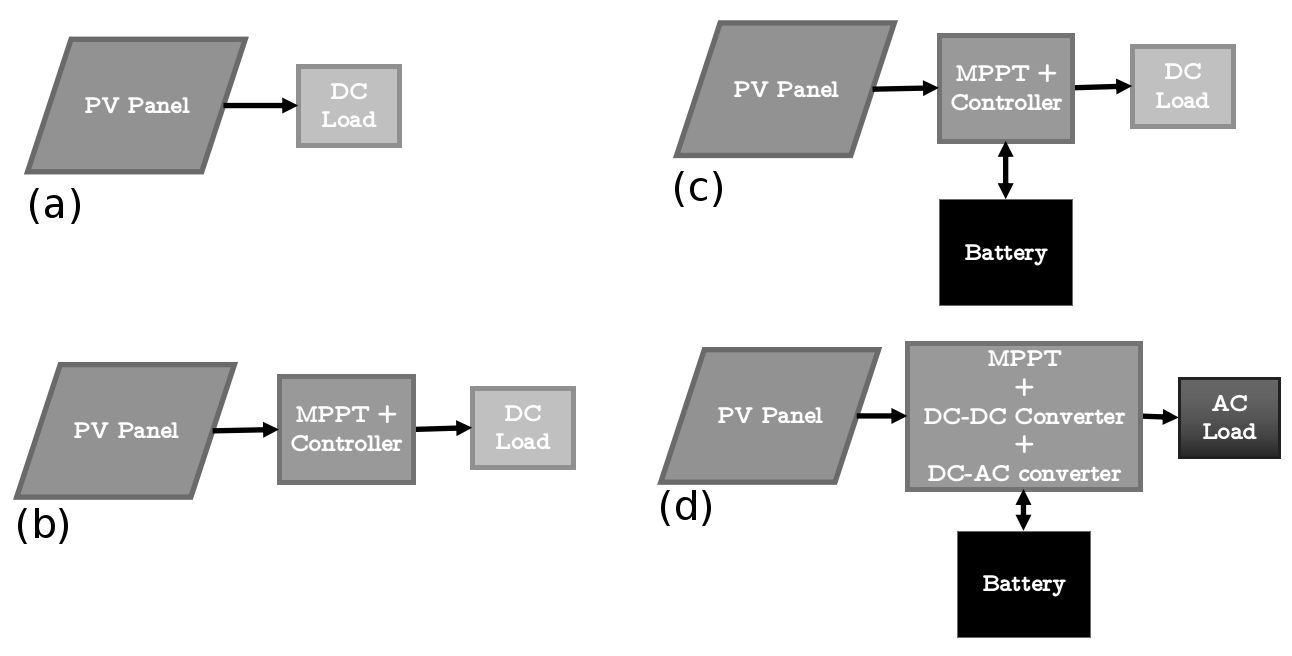
\includegraphics[width=0.5\textwidth]{reg_unreg4.png}
%\centering
%\caption{PV stand-alone systems: (a) regulated stand-alone SPV system with DC load; (b) regulated stand-alone SPV system with DC load; (c) regulated stand-alone SPV system with battery DC load; and (d) regulated stand-alone system with battery and AC load  (Source: \cite{Roy}).}
%\label{fig:standaloneSPV}
%\end{figure}

%\subsection{Regulated stand-alone PV system with DC load}
%It is similar to unregulated stand-alone system with DC load, but the main difference between this and the previous one is that this system requires a MPPT technique, as illustrated by Fig.\ref{fig:standaloneSPV} letter (b). Usually system with MPPT should have battery; otherwise, extra power will be waste.

%\subsection{Regulated stand-alone system with battery and DC load}
%Configuration with PV array, battery, MPPT and DC load, as shown in Fig.\ref{fig:standaloneSPV} letter (c). Battery is used to store the extra power of PV system. A charge controller is necessary for this type of system because the useful life of the battery is less than that of the PV module. Extra charging and deep discharging can reduce the battery life \cite{Kim}. 

%According to \cite{Pinho}, PV systems that are used to feed loads with low variation on the consumption can be sized to operate without the controller. That is called of self-regulated stand-alone PV system with battery. However, the voltage from the PV panel must be compatible with the batteries voltage. Normally, the bank of batteries are oversized related to the PV panel and to the load. The drawback is the operation of the batteries, normally overloaded or with excessive discharges (that can damage the batteries).

%\subsection{Regulated stand-alone system with battery and AC load}
%This system is similar to the previous one, but here AC load draws the power from PV system and, because of the AC load, an inverter (DC to AC converter) is required, as seen in Fig.\ref{fig:standaloneSPV} letter (d). This solution has an increase of cost because has more equipments. However, the AC availability brings the advantage of a higher number of AC appliances to use at the houses or consumer units. That configuration is the focus of the present work since it is the most common nowadays all over the world, when off-grid or isolated regions is the target.

\subsection{Design and Simulation of Solar PV systems}
%The design and validation of a PV system can be done by hand or with the aid of a software tool. 
%
In order to address different aspects of the PV system design, there are various software tools available in the literature~\cite{Rajanna,Rawat}.
%public domain and commercial software available for the PV market. 
%According to \cite{Brooks}, t
The capabilities of those tools range from simple solar resource and energy production estimation, %to site survey and system design tools,
 to complex financial analysis and project optimization. 
%Some tools also provide support to rebate programs applications and tax incentives (specific to each country or region), while other programs and worksheets focus on the technical aspects of system sizing and design.
%
%Manufacturers and integrators have yet their proprietary software to perform inverter string sizing and various system sizing and design tools, with the drawback to just include their own products among the possibilities of choice. 
Here we evaluated the most popular ones: PVWatts, SAM, HOMER, RETScreen, and Hybrid2~\cite{Pradhan,Swarnkar,NRELDobos,NRELBlair,Mills}.

%\subsection{PVWatts Calculator}
%According to \cite{Freeman} and \cite{NRELDobos}, it is a web application developed by the National Renewable Energy Laboratory (NREL), which estimates the electricity production of a grid-connected roof- or ground-mounted photovoltaic system based on a few inputs. According to \cite{NRELDobos}, to use the calculator, it is necessary to provide information about the system's location, basic design parameters, and system economics. PVWatts calculates estimated values for the system's annual and monthly electricity production, and for the electricity monetary value. This tool is suitable for very preliminary studies of a potential location for a photovoltaic system that uses crystalline silicon or thin film photovoltaic modules. The production estimates that PVWatts computation do not account for many factors that are important in the design of a photovoltaic system, therefore it is necessary support of an energy expert. The calculator estimates the monthly and annual electricity production of a photovoltaic system using an hour-by-hour simulation over a period of one year. To represent the system's physical characteristics, PVWatts requires values for six inputs: System DC size; Module type; Array type; System losses; Array tilt angle; Array azimuth angle.

%\subsection{SAM}
%SAM or System Advisor Model is a software from the U.S. Department of Energy and National Renewable Energy Laboratory. According to \cite{NRELBlair} and \cite{Cameron2008}, SAM is intended to help users to determine whether the model meets their project constraints/specifications, and (also) to provide information for readers who do not plan to use the model, but want to learn about its capabilities. SAM is a performance and financial model designed to facilitate decision making for people involved in the renewable energy industry: Project managers and engineers; Financial and policy analysts; Technology developers; and Researchers. SAM makes performance predictions and cost of energy estimates for grid-connected power projects based on installation and operating costs and system design parameters that you specify as inputs to the model. Projects can be either on the customer side of the utility meter, where they buy and sell electricity at retail rates, or on the utility side of the meter, where they sell electricity at a price negotiated through a power purchase agreement. SAM is an electric power generation model and assumes that the renewable energy system delivers power either to an electric grid, or to a grid-connected building or facility to meet electric load. It does not model thermal energy systems that meet a thermal process load. As mentioned in \cite{NRELBlair}, SAM does not model isolated or off-grid power systems, and does not model systems with electricity storage batteries.

%\subsection{HOMER}
%As defined in \cite{HOMER}, actually is a set of two tools: HOMER Legacy and HOMER Pro. HOMER is an acronym for Hybrid Optimization Model for Multiple Energy Resources. HOMER Legacy is the original HOMER software version created at the National Renewable Energy Laboratory (NREL). HOMER Legacy is a free computer model that simplifies the task of evaluating design options for both off-grid and grid-connected power systems for remote, stand-alone, and distributed generation applications. HOMER's optimization and sensitivity analysis algorithms allow the user to evaluate the economic and technical feasibility of a large number of technology options. Since 2016 HOMER Legacy can be found at HOMER web site, but only available for students and nonprofit organizations, as defined in \cite{HOMER}, and has not support available. At the short-time only the commercial version will remain.
 
%The commercial version (paid), called HOMER Pro, as defined in \cite{Swarnkar}, is a tool for optimizing micro-grid design in all sectors, from village power and island utilities to grid-connected campuses and military bases. HOMER Pro put together three tools in one product: optimization, simulation, and sensitivity analysis. HOMER Pro provides the detailed rigor of chronological simulation and optimization in a model that is intended to be easy to use. It is adaptable to a wide variety of projects. For a village or community-scale power system, HOMER can model both the technical and economic factors involved in the project. For larger systems, HOMER can provide an overview that compares the cost and feasibility of different configurations. Chronological simulation is essential for modeling variable resources, such as solar and wind power and for combined heat and power applications, where the thermal load is variable. HOMER's sensitivity analysis helps determine the potential impact of uncertain factors such as fuel prices or wind speed on a given system. 

%\subsection{RETScreen}
%As mentioned in \cite{Pradhan}, RETScreen is a decision-support tool designed to help decision makers and energy professionals to evaluate the financial viability of renewable energy, energy efficiency, and/or co-generation projects.

%RETScreen models various types of renewable energy technologies (RETs), allowing for comparisons between technology options. The software can be used to evaluate benefits from both clean energy production from power generation projects and savings through energy efficiency projects, accounting for project costs, greenhouse gas emission reductions, and financial risk. The software is freely distributed (but with restrictions to save work or print), and had three different versions:

%\begin{itemize}
%\item RETScreen 4 (discontinued, requires Microsoft Excel to run); 
%\item RETScreen Software Suit, which includes the RETScreen 4 and a Windows-based graphical software that allows project owners to verify the ongoing energy performance of their facilities (discontinued in 2013);
%\item And the actual (2016) RETScreen Expert, which allows users to evaluate energy investments over an entire project life-cycle (including benchmarking, feasibility, and performance analysis) in a fully integrated way, and within one software platform. However, this version works is only Windows-based. This version has a complete paid version, in an annual subscription way.
%\end{itemize}

%As described by \cite{Pradhan}, RETScreen performs a five-step standard analysis: setting and site conditions; energy model; cost analysis; emission analysis, financial analysis, sensitivity, and risk analysis. It is developed and maintained by the Government of Canada, through the CanmetENERGY Varennes Research Centre of Natural Resources; in collaboration with: NASA; Renewable Energy and Energy Efficiency Partnership (REEEP); United Nations Environment Programme (UNEP), and the Global Environment Facility (GEF). RETScreen is available in 36 languages; it is a multi-awarded tool, and includes equipment databases for components manufactured and available worldwide.

%\subsection{Hybrid2}
%The Hybrid2 software package, as described in \cite{Mills}, is a user-friendly tool to perform detailed long-term performance and economic analysis on a wide variety of hybrid power systems. Hybrid2 is a probabilistic/time series computer model, using time series data for loads, wind speed, solar insolation, and temperature; and the power system is designed or selected by the user, in order to predict the performance of the hybrid power system. Variations in wind speed and in load within each time step are factored into the performance predictions. The code does not consider short-term system fluctuations caused by system dynamics or component transients. This program is not supported anymore and according to \cite{UMASS}, probably after the user performs the free download of the tool, it will not work on Windows platforms later than Windows XP, what is a limitation.

Table~\ref{table:softwares} summarizes the off-the-shelf tools employed here, where only Hybrid2 does not have technical support; HOMER and Hybrid2 perform off-grid system or battery backup analysis. %all the tools perform solar photovoltaic analysis; 
Additionally, HOMER and RETScreen include economical analysis or even optimization-sensitive analysis. RETScreen and HOMER have a free web-based version, but they have limited resources since they do not allow us to save the PV projects or even upload data from manufacturers. However, commercial version of those tools, called RETScreen Expert and HOMER Pro, are available only for Microsoft Windows and the annual subscription typically range from US\$504.00 to US\$657.00.

\begin{table}[!t]
%% increase table row spacing, adjust to taste
\renewcommand{\arraystretch}{1.3}
% if using array.sty, it might be a good idea to tweak the value of
% \extrarowheight as needed to properly center the text within the cells
\caption{Comparative coverage of reference software}
\label{table:softwares}
\centering
%% Some packages, such as MDW tools, offer better commands for making tables
%% than the plain LaTeX2e tabular which is used here.
\begin{tabular}{c | c | c | c | c | c}
\hline
\hline
Characteristic  & \rotatebox{90}{PVWatts} & \rotatebox{90}{SAM} & \rotatebox{90}{HOMER} & \rotatebox{90}{RETScreen} & \rotatebox{90}{Hybrid2}\\
\hline
\hline
Support & X & X & X & X &  \\
\hline
Off-grid systems &   &   & X & X & X\\
\hline
Hybrid systems &  &  & X & X & X\\
\hline
Photovoltaics & X & X & X & X & X\\
\hline
Batteries &  &  & X &  & X\\
\hline
\makecell{Main technical (T) \\ or economical(E)} & T & T & E & E & T \\
\hline
Optimization &  &  & X & X &  \\
\hline
Sensitive analysis &  &  & X & X & \\
\hline
\hline
\end{tabular}
\end{table}

%-------------------------------------------------------------------
%\subsection{Paper Proposal x Reference Tools}
%-------------------------------------------------------------------
%
In this study, only HOMER remains for a comparative evaluation with our proposed verification approach. %All tools need some parameters inherently from manufacturer's catalog.
%, so the project starts with manufacturers and integrators tool to define the basic items of the project: panels, inverters, controllers, and batteries. 
%After that, the potential solution is analyzed in another tool to simulate or even optimize the proposed solution. Therefore, that is 
Thus, the main challenge here is to demonstrate the application of software model checking to formally verify a stand-alone PV solution, thus proving that this approach is more effective and complete than other state-of-the-art tool such as HOMER Pro. The comparative evaluation between HOMER Pro and our approach is presented in Section~\ref{sec:results_indeed}.

%-------------------------------------------------------------------
\subsection{Component models for a stand-alone PV system }
%-------------------------------------------------------------------

%The main purpose of this section is to describe the models for the elements of a stand-alone PV system: PV generator, battery, controller, inverter, and load. 
The mathematical modeling of the PV system is based on modular blocks, as illustrated in Fig.\ref{fig:blockdiagram}. It identifies the PV generator, batteries, charge controller, inverter, and AC load. 

The PV generator, which can be a panel or an array, is a semiconductor device that can convert solar energy into DC electricity. In Fig.\ref{fig:blockdiagram}, there are two variables that depend on the site where the system is deployed and the weather (i.e., solar irradiance $G$ and temperature $T$). For night hours or rainy days, we need to hold batteries, where power can be stored and used. The use of battery as a storage form implies the presence of a charge controller~\cite{Hansen,Mellit}. The PV arrays produce DC and therefore when the PV system contains an AC load, a DC/AC conversion is required. That converter is called of inverter; and the AC load dictates the behavior of AC electrical load from the house that will be fed by the system.
%
%The modular structure facilitates the modeling of the other system structures and replacement of elements, such as a DC load instead of an AC load. 
%
\begin{figure}[h]
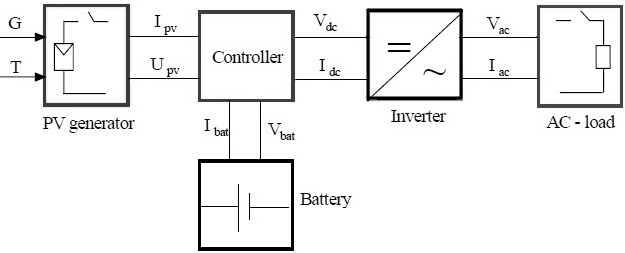
\includegraphics[width=0.48\textwidth]{blockdiagramPVS2}
\centering
\caption{Block diagram for a typical stand-alone PV system~\cite{Hansen}.}
\label{fig:blockdiagram}
\end{figure}

%In the literature, there are several mathematical models available for each component of PV systems. At the next section, the mathematical model for each component is presented. 

%-------------------------------------------------------------------
\subsection{PV generator model}
\label{sec:PVmodel}
%-------------------------------------------------------------------

%A photovoltaic PV generator is the whole assembly of solar cells, connections, protective parts, and supports. 
%In the present modeling, the focus is only on cell/module/array.
%
%%%%%%The basic element of a PV system is a PV cell, also called a solar cell. A solar cell is a semiconductor device that can convert solar energy into DC electricity. 
%The semiconductor materials (usually silicon), which are specially treated to form an electric field, positive on one side (backside) and negative on the other (towards the sun). When solar energy (photons) hits the solar cell, electrons are knocked loose from the atoms in the semiconductor material, creating electron-hole pairs \cite{Lorenzo}. If electrical conductors are attached to the positive and negative sides, forming an electrical circuit, the electrons are captured in the form of electric current $ I_{ph} $ (photocurrent).
%%%%%To increase their utility, a number of individual PV cells are interconnected together in a %sealed, weatherproof 
%%%%%package called panel or module. 

%For instance, a 12 V Panel will have 36 cells connected in series and a 24 V Panel will have 72 PV cells connected in series. In addition, to achieve the desired voltage and current, modules are wired in series and parallel into what is called a PV Array, as shown in Fig.\ref{fig:celmodarray}. The flexibility of the modular PV system allows designers to create PV systems that can meet a wide variety of electrical demands. 
%
%\begin{figure}[h]
%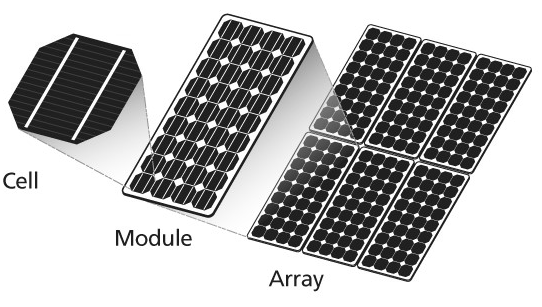
\includegraphics[width=0.4\textwidth]{celmodarray}
%\centering
%\caption{PV cell, module and array (Source: \cite{SamlexSolar})}
%\label{fig:celmodarray}
%\end{figure}
%
%%%%%The PV modules are generally rated under standard test conditions (STC), and the parameters required for the input of the PV modules are relying on meteorological conditions.
%the meteorological conditions of the area to be serviced by PV solution. %However, the climatic conditions are unpredictable due to the random nature of their occurrence \cite{Jakhrani}.
%, which leads to the following specification by the manufacturers:  solar radiation of 1000 W/m$^{2}$, cell temperature of 25$^{o}$C, and solar spectrum of 1.5. The parameters required for the input of the PV modules are relying on the meteorological conditions of the area to be serviced by photovoltaic solution. However, the climatic conditions are unpredictable due to the random nature of their occurrence \cite{Jakhrani}.
%
%These uncertainties lead to either over- or underestimation of energy yield from PV modules. An overestimation up to 40\% was reported as compared to the rated power output of PV modules \cite{Durisch}. The growing demand of photovoltaics technologies led to research in the various aspects of its components from cell technology to the modeling, size optimization, and system performance \cite{Yatimi}, \cite{Saloux}, \cite{Mellit}. 
%
%Modeling PV modules is one of the major components responsible for proper functioning of PV systems. However, the estimation of models is affected by various intrinsic and extrinsic factors, which ultimately influence the behavior of current and voltage. Therefore, perfect modeling is essential to estimate the performance of PV modules in different environmental conditions \cite{Jakhrani}.
% 
%Modeling provides the ways to understand the current, voltage, and power relationships of PV systems.
  
The performance of PV systems %, %that is, the output current/voltage curve ($I-V$ curve), 
is usually studied using an equivalent circuit model~\cite{Yatimi,Saloux,Mellit}, which consists of a current source with one or two diodes connected in parallel, and up to two resistors, one connected in parallel and the other one in series, to take into account energy losses in this model~\cite{Cubas}. 
%Based on these electronic components, four basic configurations are normally used when studying photovoltaic systems, as shown by Fig. \ref{fig:equivckt}. 
\begin{figure}[h]
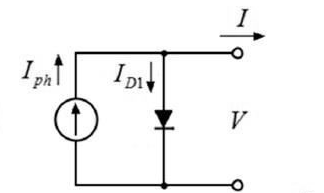
\includegraphics[width=0.20\textwidth]{equivckt1D}
\centering
\caption{1-diode equivalent PV cell/panel circuit model~\cite{Cubas}.}
%\caption{Four different equivalent circuit models: (a) 1-diode; (b) 1-diode/1-resistor; (c) 1-diode/2-resistor; (d) 2-diode/2-resistor (Source: \cite{Cubas})}
\label{fig:equivckt}
\end{figure}
 
The 1-diode model, illustrated in Fig. \ref{fig:equivckt}, whose equation relates the output current, $I$, to the output voltage, $V$, is described by Eq.~\eqref{eq:1diodemodel}:
\begin{equation}
\label{eq:1diodemodel}
I = I_{ph}-I_{D1}=I_{ph}-I_{0}\left[ exp \left( \dfrac{V}{NaV_{T}} \right)  \right], 
\end{equation}

\noindent where $I_{ph}$ is the photocurrent delivered by the constant current source; $I_{0}$ is the reverse saturation current corresponding to the diode; $N$ is the number of series-connected cells ($N=1$ in a single cell configuration); $a$ is the ideality factor (or quality factor) that takes into account the deviation of the diodes from the Shockley diffusion theory ($a=1$ for ideal diodes and between $1$ and $2$ for real diodes); $V_{T}$ is the thermal voltage ($ V_{T}=k_{B}T/q $); $ k_{B} $ is the Boltzmann constant ($ 1.3806503\times10^{-23}J $); $T$ the temperature of the p-n junction (or cell temperature) in Kelvin; $q$ is absolute value of the electron's charge ($ -1.60217646\times10^{-19}C $).

%\begin{itemize}
%\item $I_{ph}$ is the photocurrent delivered by the constant current source; 
%\item $ I_{0} $ is the reverse saturation current corresponding to the diode; 
%\item $ N $ is the number of series-connected cells in the photovoltaic system to be analyzed; $ N=1 $ in a single cell configuration.
%	\begin{itemize}
%	\item $ N=1 $ in a single cell configuration. 	
%	\end{itemize}	  
%\item $ a $ is the ideality factor (or quality factor) that takes into account the deviation of the diodes from the Shockley diffusion theory; $a=1$ for ideal diodes and between $ 1 $ and $ 2 $ for real diodes.
%	\begin{itemize}
%	\item $a=1$ for ideal diodes and between $ 1 $ and $ 2 $ for real diodes. 	
%	\end{itemize}
%\item $V_{T}$ is the thermal voltage ($ V_{T}=k_{B}T/q $);
%	\begin{itemize}
%	\item $ k_{B} $ is the Boltzmann constant ($ 1.3806503\times10^{-23}J $); 
%	\item $ T $ the temperature of the p-n junction (or cell temperature) expressed in Kelvin; 
%	\item $ q $ is absolute value of the electron's charge ($ -1.60217646\times10^{-19}C $).	
%	\end{itemize}	 
%\end{itemize}
%
%This model has only three unknown parameters ($ I_{ph}$, $I_{0}$, and $a $), and it assumes that the series resistance is $ zero $ and shunt resistance is $ infinite $ and, thus, both of these parameters are ignored.
%
%The 1-diode/1-resistor model, is described by Equation \ref{eq:1d1rmodel}. 
%
%\begin{equation}
%\label{eq:1d1rmodel}
%I =I_{ph}-I_{0}\left[ exp \left( \dfrac{V+IR_{s}}{NaV_{T}} \right) -1 \right] 
%\end{equation}
%
%Where $R_{s}$ is the series resistor.
%
%At this model, there are four unknown parameters ($ I_{ph}$, $I_{0}$, $ R_{s} $, and $ a $), and it assumes shunt resistance as $ infinite $.
%
%The 1-diode/2-resistor model, is described by Equation \ref{eq:1d2rmodel}. 
%
%\begin{equation}
%\label{eq:1d2rmodel}
%I =I_{ph}-I_{0}\left[ exp \left( \dfrac{V+IR_{s}}{NaV_{T}} \right) -1 \right] - \dfrac{V+IR_{s}}{R_{sh}}
%\end{equation}
%
%Where $R_{sh}$ is the shunt resistor.
%
%At this model, there are five unknown parameters ($ I_{ph}$, $I_{0}$, $ R_{s} $, $ R_{sh} $, and $ a $).
%
%And the 2-diode/2-resistor model, is described by Equation \ref{eq:2d2rmodel}. 
%
%\begin{multline}
%\label{eq:2d2rmodel}
%I =I_{ph}-I_{01}\left[ exp \left( \dfrac{V+IR_{s}}{Na_{1}V_{T}} \right) -1 \right] - \\ %I_{02}\left[ exp \left( \dfrac{V+IR_{s}}{Na_{2}V_{T}} \right) -1 \right] - \dfrac{V+IR_{s}}{R_{sh}}
%\end{multline}
%
%This model has six unknown parameters with two exponential terms. 
%Briefly, both single and double diode models require the knowledge of all unknown parameters, which is usually not provided by manufacturers. Nevertheless, the current-voltage equation is a transcendental expression \cite{Jakhrani}.  
%
%However, regardless of the adopted model, the parameters of the equations must be estimated to adapt the corresponding model to the real behavior of the solar cell/panel. 
%
%For that reason, researchers gradually focused on searching out the approximate methods for the calculation of unknown parameters and walked through three different paths. The analytical methods give exact solutions by means of algebraic equations, as done by \cite{Cubas} and \cite{Brano}. However, due to implicit nature and nonlinearity of PV cell or module characteristics, it is hard to find out the analytical solution of all unknown parameters, as described by \cite{Hasan}. Thus, numerical methods such as Newton-Raphson method or Levenberg-Marquardt algorithm were preferred, as described by \cite{Mellit}. This happens because numerical methods give approximate solution of the nonlinear problems without searching for exact solutions. However, numerical methods are time consuming and need long term time series data, which is not available in developing countries. \cite{Jakhrani} did a mixed methodology using analytical and numerical steps together.  \cite{Shenawy} create a method to discover the unknown parameters of the PV panels through experimentation (essays). And \cite{Tian} did a mix of analytical and experimental methodology to get the unknown parameters, but samples of the PV modules are necessary to perform some essays, when we use experimental technique. 

%Therefore, a wide variety of models exists for estimation of power output of PV modules (and $I-V$ or $P-V$ curves). However, the present work will rely on t
The simplified model of 1-diode has demonstrated that it has a small error rate, between 0.03\% and 4.68\% from selected PV panels tested~\cite{Saloux}. In addition, this mathematical modeling has the advantage of being an explicit model, which does not use iterative numerical calculation, which is time-consuming to computing~\cite{Cubas}. 
 %
%\subsection{PV Panel Model}
%With the proposed model, an explicit set of equations is derivate from the ideal PV model given by Equation \ref{eq:1diodemodel}.
%
%A single-diode without series and shunt resistances is considered. 
Eq.~\eqref{eq:1diodemodel} is used to express currents and voltages at each key point of the characteristic curve from a PV cell \cite{Villalva}.
% shown in Fig. \ref{fig:ivcurve}.
%
%\begin{figure}[h]
%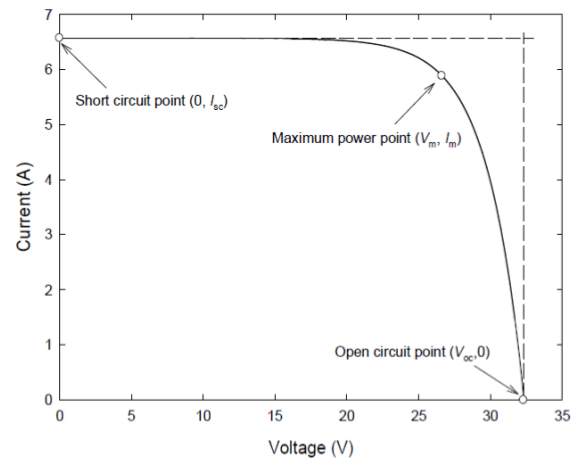
\includegraphics[width=0.4\textwidth]{ivcurve}
%\centering
%\caption{$ I-V $ characteristic curve of an ideal PV cell (Source: \cite{Saloux})}
%\label{fig:ivcurve}
%\end{figure}
%
%Hence, the short-circuit current, the open-circuit voltage, the maximum power voltage and current are written as defined by \cite{Saloux} and shown from Equations \ref{eq:Isc} to \ref{eq:Im}.
%\begin{equation}
%\label{eq:Isc}
%I_{sc}=I_{ph}\vert_{V=0}
%\end{equation}
%
%\begin{equation}
%\label{eq:Voc}
%V_{oc}=\dfrac{aNk_{B}T}{q}ln\left( 1+\dfrac{I_{sc}}{I_{0}} \right) 
%\end{equation}
%
%\begin{equation}
%\label{eq:exp}
%exp\left( \dfrac{qV_{oc}}{aNk_{B}T} \right) = \left(1+\dfrac{qV_{m}}{aNk_{B}T} \right) exp \left( \dfrac{qV_{m}}{aNk_{B}T} \right) 
%\end{equation}
%
%\begin{equation}
%\label{eq:Im}
%I_{m} =I_{ph}-I_{0}\left[ exp \left( \dfrac{qV_{m}}{aNk_{B}T} \right) -1 \right] 
%\end{equation}
%
%Equation \ref{eq:exp} is not explicit with the PV key parameters, therefore need to be rewritten in a different way. 
%
%A PV cell has a hybrid behavior, i.e., a current-source at the short-circuit point and voltage-source at the open-circuit point \cite{Saloux}. 
%These two regions are characterized by two asymptotes of the $ I-V $ curve in Fig. \ref{fig:ivcurve}, where the transition is a compromise between both behaviors. It is interesting to observe that the maximum power point corresponds to a trade-off condition, where the current is still high enough before it starts decreasing with increasing the output voltage (Fig. \ref{fig:ivcurve}).
%
%Based on this, the tangent of the I-V curve can be used to evaluate the transition between current- to voltage-source controlled regions; this operation yields Equation \ref{eq:didv}.
%
%\begin{equation}
%\label{eq:didv}
%\dfrac{dI}{dV}=-\dfrac{qI_{0}}{aNk_{B}T}exp \left( \dfrac{qV}{aNk_{B}T}  \right) 
%\end{equation}
%
%The derivative of Equation \ref{eq:didv} is used to calculate the output voltage that corresponds to the maximum power operation condition of the cell. Therefore, the Equation \ref{eq:Vmderiv} is generated.
%
%\begin{equation}
%\label{eq:Vmderiv}
%V_{m}=\dfrac{aNk_{B}T}{q} ln \left( -\dfrac{qNk_{B}T}{qI_{0}} \left( \dfrac{dI}{dV}  \right)_{V_{m}}   \right) 
%\end{equation}
%
%It is evident that Equation \ref{eq:Vmderiv} requires an expression of the derivative of the current with voltage evaluated at the maximum power point. The fact that the maximum power corresponds to an extreme, the variation of the maximum output power with voltage is relatively small, i.e., a change on $ V_{m} $ has a relatively small effect on the maximum power of the cell \cite{Saloux}. Consequently, considering the asymptotic behavior of the $I-V$ curve at short- and open-circuit conditions, the derivative required by Equation \ref{eq:Vmderiv} can be calculated as shown in Equation \ref{eq:dIdV_Vm}.
%
%\begin{equation}
%\label{eq:dIdV_Vm}
%\dfrac{dI}{dV}\vert_{V_{m}} \cong -\dfrac{0-I_{sc}}{V_{oc}-0}=\dfrac{I_{sc}}{V_{oc}}
%\end{equation}
%
%Replacing the Equation \ref{eq:dIdV_Vm} into Equations \ref{eq:Vmderiv} and \ref{eq:Im}, 
%
The voltage and the current at the maximum power point tracking (MPPT), can be described by Equations \eqref{eq:Vmfinal}, \eqref{eq:Imfinal}, and \eqref{eq:Pm}  as follows~\cite{Saloux}: %These equations are used to calculate the key cell parameters at the maximum power point as function cell temperature and parameters from the manufacturer's data-sheet.
\begin{equation}
\label{eq:Vmfinal}
V_{m}=\dfrac{aNk_{B}T}{q} ln \left( \dfrac{aNk_{B}T}{qI_{0}} \dfrac{I_{sc}}{V_{oc}}  \right). 
\end{equation}

\begin{equation}
\label{eq:Imfinal}
I_{m} = I_{ph} + I_{0} - \dfrac{aNk_{B}T}{q} \left( \dfrac{I_{sc}}{V_{oc}} \right).  
\end{equation}

\begin{equation}
\label{eq:Pm}
P_{m} = V_{m} I_{m}.
\end{equation}

%\begin{multline}
%\label{eq:Pm}
%P_{m} = V_{m} I_{m} = \left[ \dfrac{aNk_{B}T}{q} ln \left( \dfrac{aNk_{B}T}{qI_{0}} \dfrac{I_{sc}}{V_{oc}}  \right) \right] \times \\ \left[ I_{ph} + I_{0} - \dfrac{aNk_{B}T}{q} \left( \dfrac{I_{sc}}{V_{oc}} \right)  \right] 
%\end{multline}
%
However, the photocurrent delivered by the constant current source ($I_{ph}$) or even the reverse saturation current ($ I_{0} $) are not given by PV manufacturers. Therefore, Eq.~\eqref{eq:Iph} is used to calculate the photocurrent as function of irradiance and temperature~\cite{Villalva}:
\begin{equation}
\label{eq:Iph}
I_{ph}=\dfrac{G}{G_{ref}} \left[ I_{ph,ref} + \mu_{I} \left( T-T_{ref} \right)    \right], 
\end{equation}

\noindent where the reference state (STC) of the cell is given by the solar irradiance $ G_{ref}=1000 W/m^{2} $ and the temperature $ T_{ref}=298.15 K (=25^{o}C) $; $ \mu_{I} $ is the short-circuit current temperature coefficient ($A/K$) %and corresponds to the photocurrent obtained from a given PV cell working at reference conditions 
(provided by PV manufacturers). $ I_{ph,ref} $ can be approximated to the reference short-circuit current \cite{Jakhrani} that is provided by PV manufacturers ($ I_{sc,ref} $).
%
The cell temperature ($ T $) is described by Eq.~\ref{eq:Tcell}~\cite{Ross}:
\begin{equation}
\label{eq:Tcell}
T = T_{air} + \dfrac{NOCT-20}{800}G,
\end{equation}

\noindent where $ T_{air} $ is the ambient temperature, $NOCT$ is the nominal operating cell temperature (in $^{o}$C) that is found at the PV manufacturer's data-sheet \cite{Ross}, and $G$ is the solar irradiance ($ W/m^{2} $) of the place where the PV system is deployed.

Furthermore, Eq.~\eqref{eq:I0} permits the saturation current ($ I_{0} $) to be expressed as a function of the cell temperature as~\cite{Villalva} 
%In this study, this relation is explicitly written based on cell open-circuit conditions using the short-circuit current temperature coefficient as well as the open-circuit voltage temperature coefficient (Equation \ref{eq:I0}).

\begin{equation}
\label{eq:I0}
I_{0} = \dfrac{I_{sc,ref} + \mu_{I}(T - T_{ref})}{exp \left[ \dfrac{q(V_{oc,ref} + \mu_{V} (T - T_{ref}))}{aNk_{B}T}    \right] -1},
\end{equation}

\noindent where $ V_{oc,ref} $ is the reference open-circuit voltage and $ \mu_{V} $ is an open-circuit voltage temperature coefficient ($ V/K $).

%The ideality (or quality) factor of the diode $ a $, which is usually considered as a constant \cite{Villalva}, is determined in the reference state. 
Using the maximum power point current (cf. Eq.~\eqref{eq:Pm}) and the saturation current in the reference temperature given by Eq.~\eqref{eq:I0}, the diode ideality factor is determined by Eq.~\eqref{eq:a}:
\begin{equation}
\label{eq:a}
a = \dfrac{q(V_{m,ref}-V_{oc,ref})}{Nk_{B}T} \dfrac{1}{ln \left( 1 - \dfrac{I_{m,ref}}{I_{sc,ref}}  \right) },
\end{equation}

\noindent where $V_{mref}$, $V_{oc,ref}$, $I_{m,ref}$, and $I_{sc,ref}$ are key cell values obtained under both actual cell temperature and solar irradiance conditions, usually provided by manufacturers; the PV generator model is now completely determined.
%; it requires the actual cell temperature (or the air temperature), the actual solar irradiance and common data provided by manufacturers.
%
%If the PV cells are in parallel, then there is a parallel array. Therefore, there will be a change at the $ I_{ph} $ and $ I_{0} $and the resulting current is given by Equation \ref{eq:Iarray}, as demonstrated in \cite{Saloux}.
%
%\begin{equation}
%\label{eq:Iarray}
%I_{array} = (N_{cells in parallel})(I_{one cell})
%\end{equation}
%
%Where $ I_{one cell} $ is the current from Equation \ref{eq:Imfinal}.
%
%In addition, if the panels are in series, the current do not change but the total voltage is the sum of the each panel's voltage.
%
%\begin{equation}
%\label{eq:Varray}
%V_{array} = (N_{cells in series})(V_{one panel})
%\end{equation}
%
%Where $ V_{one panel} $ is the voltage from Equation \ref{eq:Vmfinal}.

In addition to the model verification performed by the proposed technique, there is the prior stage of PV system sizing check, based on manufacturer's data and information from the sizing and the site; this stage ensures that the system meets its specification, thereby considering the standard project steps~\cite{Pinho}.
%
Firstly, we need to correct the energy consumption estimated to the load ($E_{consumption}$), which is carried out by Eq.~\eqref{eq:Ecorrected}~\cite{Pinho}, where the efficiency of batteries ($\eta_{b}$), controller ($\eta_{c}$), and the inverter ($\eta_{i}$) are considered as
\begin{equation}
\label{eq:Ecorrected}
E_{corrected} = \dfrac{E_{consumption}}{ \eta_{b} \eta_{c} \eta_{i} }.
\end{equation}

The total minimum number of needed solar panels ($N_{TPmin}$) is computed by Eq.~\eqref{eq:NTPmin} and the check is performed using Eq.~\eqref{eq:NTP}, where the sized number of panels ($ N_{TP} $) must be greater than the result from Eq.~\eqref{eq:NTPmin}.
\begin{equation}
\label{eq:NTPmin}
N_{TPmin} = \dfrac{E_{corrected}}{E_{p}}.
\end{equation}

\begin{equation}
\label{eq:NTP}
N_{TP} \geq N_{TPmin}.
\end{equation}

Particularly, the total number of panels in series ($N_{PSmin}$) and parallel ($N_{PPmin}$) are given by~\eqref{eq:NPSmin} and \eqref{eq:NPPmin}, respectively. With the check performed by (\ref{eq:NPS}) and (\ref{eq:NPP}), $ V_{system} $ is the DC voltage of the bus, normally $12$, $24$ or $48$ V.
\begin{equation}
\label{eq:NPSmin}
N_{PSmin} = \dfrac{V_{system}}{V_{m,ref}}.
\end{equation}

\begin{equation}
\label{eq:NPPmin}
N_{PPmin} = \dfrac{N_{TPmin}}{N_{PSmin}}.
\end{equation}

\begin{equation}
\label{eq:NPS}
N_{PS} \geq N_{PSmin}.
\end{equation}

\begin{equation}
\label{eq:NPP}
N_{PP} \geq N_{PPmin}.
\end{equation}

%------------------------------------------------------------
\subsection{The Battery Storage Model }
\label{sec:BATmodel}
%------------------------------------------------------------

%Because of the fluctuating nature of the output delivered by the PV arrays, batteries are nece\sqrt{•}ry in a PV system. Thus, during the hours of sunshine, the PV system feeds directly the load and the excess electrical energy is stored in the battery. During the night, or during a period with low solar irradiation, energy is supplied to the load from the battery \cite{Mellit}.
  
Various models have been described in the literature and the most common ones are based on lead-acid batteries~\cite{Copetti,Manwell93,Pinho};
%, and \cite{Manwell94}. 
%However, regardless of the model, normally the following parameters are required: 
%
%\begin{itemize}
%\item Nominal capacity ($ q_{max} $), is the number of Ampere-hours ($ Ah $) that can maximally be extracted from the battery
%, under predetermined discharge conditions.
%\item State of charge ($ SOC $), is the ratio between the present capacity and the nominal capacity, i.e., $ SOC = q/q_{max} $. 
%Obviously $ 0<SOC<1 $. 
%If $ SOC=1 $, then the battery is totally charged; and if $ SOC=0 $, the battery is fully discharged
%\item Charge (or discharge) regime.This parameter reflects the relationship between the nominal capacity of a battery and the current at which it is charged (or discharged). 
%It is expressed in hours: for instance, discharge regime is 30h for a battery of 150 Ah that is discharged at 5A.
%\item Efficiency ($\eta_{b}$), is the ratio of the charge extracted during discharge divided by the amount of the charge needed to restore the initial state of charging or discharging current. 
%\item Lifetime, is the number of charge/discharge cycles the battery can sustain before losing 20\% of its nominal capacity.
%\end{itemize}
%
%The merit of a stand-alone PV system is evaluated in terms of the reliability of the electricity supply to the load and in terms of the long-term efficiency of the components. The battery efficiency was described in this section, and the liability is quantified by the concept of loss of load probability (LLP). LLP is defined as the ratio between the Ampere-hour deficit and the Ampere-hour demand, both with respect to the load, over a long period of time \cite{Copetti}. 
%
%In general, the battery models view the battery as a voltage source $ E $ in series with an internal resistance $ R_{0} $, as shown in Fig. \ref{fig:batteryckt}. 
%
%\begin{figure}[h]
%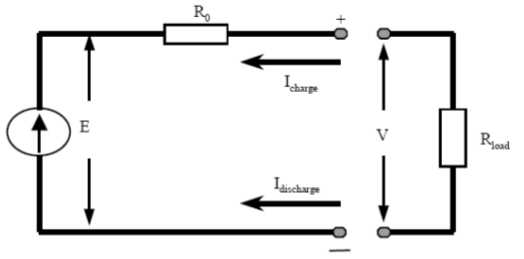
\includegraphics[width=0.4\textwidth]{batteryckt}
%\centering
%\caption{Schematic diagram of the battery (Source: \cite{Hansen})}
%\label{fig:batteryckt}
%\end{figure}
%
%The terminal voltage of the battery can be expressed in terms of its open circuit voltage and the voltage across the internal resistance of the battery \cite{Sukamongkol}, as shown by Equation 31.  
%
%Where $ V_{b} $ is the battery terminal voltage, $ E_{oc} $ is the battery circuit voltage, $ I_{b} $ is the battery current, and $ R_{b} $ is the internal resistance of the battery.
%
%The battery model, which describes the relationship between the voltage, current and the state of charge, can be found in \cite{Copetti}, \cite{Manwell93}, and \cite{Manwell94}.  
%
%The Kinetic Battery Model (KiBaM) of Manwell and McGowen \cite{Manwell93} was developed at the University of Massachusetts to predict the performance of the battery, based on manufacturer's data. However, it uses some data extracted from tested batteries in laboratory. Therefore is not suitable to this study. 
%
that kind of battery has relative low cost and wide availability~\cite{Copetti}. 
%
Here, the model adopted uses only manufacturer's data without empirical tests~\cite{Copetti}. % and allows finding relations among voltage, current, state of charge and temperature. 
%
The discharge voltage equation is described by \eqref{eq:bat_Vd} as
%The first term represents the voltage variation with the state of charge ($ SOC $), i.e., the electrolyte concentration, and the second is the variation due to internal resistance variation.
%
\begin{multline}
\label{eq:bat_Vd}
V_{d} = \left[ 2.085-0.12(1-SOC) \right] - \\ \dfrac{I}{C_{10}} \left( \dfrac{4}{1+I^{1.3}} + \dfrac{0.27}{SOC^{1.5}}+0.02 \right) (1-0.007 \Delta T),
\end{multline}

\noindent where $C_{10}$ means 10h of rated capacity, which is standard on the manufacturer's data-sheet, $\Delta T$ is temperature variation ($\Delta T=T-T_{ref} $, $ T_{ref}=25^{o}C $), $ SOC $ or state of charge indicates how much electric charge is stored in the cell at a given time. Mathematically, it is the ratio between the present capacity and the nominal capacity (in $ Ah $, provided by manufacturer). If $SOC=1$, then the battery is totally charged; and if $ SOC=0 $, then the battery is fully discharged.  %, defined by Equation \ref{eq:SOCbat}.
%\begin{equation}
%\label{eq:SOCbat}
%SOC = \left( 1 - \dfrac{Q}{C} \right) 
%\end{equation}
%
%Where $ Q $ is the charge delivered at the time of interest ($ Q=It $), and C is the battery capacity.
%
%The ratio between $ Q $ and $ C $ represents t
The depth of discharge ($DOD$) or the fraction of discharge, is $DOC=1-SOC$.

%The efficiency of the battery discharge is assumed to be 100\%, according \cite{Copetti}; however, the total amount of useful charge available during discharge is limited by the current rate and temperature given by Equation \ref{eq:CC10}. This equation, called of capacity, is normalized with respect to discharge current corresponding to $ C_{10} $ rated capacity ($ I_{10} $).
%
%\begin{equation}
%\label{eq:CC10}
%\dfrac{C}{C_{10}} = \dfrac{1.67}{1+0.67 \left( \dfrac{I}{I_{10}} \right)^{0.9} }(1+0.005 %\Delta T)
%\end{equation}
%
%Note that when the discharge current tends to zero at 25$^{o}$C, the maximum capacity that can be removed is about 67\% over the capacity.

For the charging process, however, the parameters are described by Eq.~\eqref{eq:Vcbat} as
%
\begin{multline}
\label{eq:Vcbat}
V_{c} = [2+0.16SOC]+ \\ \dfrac{I}{C_{10}} \left( \dfrac{6}{1+I^{0.86}} + \dfrac{0.48}{(1-SOC)^{1.2}} + 0.036  \right) (1-0.025 \Delta T).
\end{multline}

Note that SOC can be calculated easily at any point during the discharge period, thereby considering the current drained from batteries during a certain time period. %; however, during recharge it is much more difficult \cite{Copetti}.
%Generally, the efficient region is where $ SOC $ is below $ 0.7 $ and $ V_{c} $ is less than $2.3 V$ per cell. The efficiency drops to zero at full charge and the function that represents the charge efficiency ($ \eta_{c} $) variation with state of charge and current rate is given in Equation \ref{eq:efficcharge}.
%\begin{equation}
%\label{eq:efficcharge}
%\eta_{c} = 1 - exp \left[ \dfrac{20.73}{\dfrac{I}{I_{10}}+0.55} (SOC-1) \right] 
%\end{equation}
%
%\cite{Copetti} show that, 
%During overcharge, gassing occur and tests demonstrated that the final charge voltage ($ V_{ec} $) increases with the current intensity and with the decreasing of the temperature (\ref{eq:Vec}). It was created a function for the gassing voltage as well, as shown in (\ref{eq:Vg}). In addition, the overcharge phenomenon can be represented by (\ref{eq:Voverc}).
%\begin{equation}
%\label{eq:Vec}
%V_{ec} = \left[ 2.45 + 2.011 ln \left( 1+\dfrac{I}{C_{10}} \right)  \right] (1-0.002 \Delta T)
%\end{equation}
%
%\begin{equation}
%\label{eq:Vg}
%V_{g} = \left[ 2.24 + 1.97 ln \left( 1+\dfrac{I}{C_{10}} \right)  \right] (1-0.002 \Delta T)
%\end{equation}
%
%\begin{multline}
%\label{eq:Voverc}
%V_{c} = V_{g} + (V_{ec} - V_{g}) \\ \left[ 1- exp \left( \dfrac{Ah_{restored}-0.95C}{I\tau}  \right)    \right] 
%\end{multline}
%
%Where $ Ah_{restored} $ represents the Ampere-hour stored in the battery with regard to the battery capacity ($ C $) during this hour.
%
%The function assumes that 95\% of the capacity was already restored at the start of overcharge.
%
%The time constant of the phenomenon ($ \tau $) is reversely proportional to the charge intensity and can be written by (\ref{eq:tau}).
%\begin{equation}
%\label{eq:tau}
%\tau = \dfrac{17.3}{1+852 \left( \dfrac{I}{C_{10}} \right) ^{1.67} }
%\end{equation}
%
%Therefore, to model the voltage ($ V_{c} $) evolution of the battery, (\ref{eq:Vcbat}) can be used up the start of gassing ($ V_{c} \leq V_{g} $). And during overcharging ($ V_{c} > V_{g} $), (\ref{eq:Voverc}) can be used until a constant final voltage ($ V_{ec} $) is reached.
%
%The storage capacity of the battery can be calculated using Equation \ref{eq:stor}, as defined in \cite{Wenham}.
%
%\begin{equation}
%\label{eq:stor}
%Storage capacity = \dfrac{N_{C}E_{load}}{DOD \eta _{b}}
%\end{equation}
%
%Where $ DOD $ is the maximum possible depth of battery discharge, $ E_{load} $ is the average energy consumed by the load, $ N_{C} $ is the largest number of continuous cloudy days of the area, and $ \eta_{b} $ is the efficiency of the battery.
%
%As an example of this formula application, as shown by \cite{Abdulateef}, considering that a stand-alone PV system is intended to supply $1.5 kW/48 V$ for 24 hours ($=36 kWh$); The largest number of continuous cloudy days in the selected site is about 1 day; For a maximum depth of discharge for the battery $DOD$ of $0.8$ and battery efficiency $80\%$.
%
%Then the storage capacity using Equation \ref{eq:stor} becomes $56.3 kWh$. Since the selected DC bus voltage is $48 V$, then the required Ampere-hours of the battery is $1173 Ah$ ($56.3 kWh/48$). If a single battery of 12 V and 350 Ah is considered, then four batteries are connected in series ($4 \times 350 Ah = 1400 Ah$).
%
%At this research, it was considered a simplified model for charging (Equation \ref{eq:charge}) and discharging (Equation \ref{eq:discharge}) of the batteries, even considering that the process is not linear and depends on the temperature. The equations are used to update the $SOC$ of the batteries, and have the number of hours ($ Num_{h} $) as a variable. There is a factor (1.15) which is present at the charging equation, and is necessary to express that during the charging process is usual to reach 115\% of the battery capacity
%
%\begin{multline}
%\label{eq:charge}
%SOC_{charge} = SOC_{previous} + \\ \dfrac{100*Pm*Num_{h}}{V_{system}*capacity*N_{BP}*1.15}
%\end{multline}
%
%\begin{multline}
%\label{eq:discharge}
%SOC_{discharge} = SOC_{previous} - \\ \dfrac{100*I_{drained}*Num_{h}}{capacity}
%\end{multline}
%
%
In addition to the model verification, there is also the prior stage of project sizing check, as performed for the solar panel. Firstly we define the total capacity of the battery bank, as described by Eq. \eqref{eq:Cbank} as
\begin{equation}
\label{eq:Cbank}
C_{bank} = \dfrac{E_{corrected} \times autonomy}{V_{system} \times DOD}.
\end{equation}
%
\noindent where the variable $autonomy$ is a design definition and normally has a value ranging from $6$ to $48$h; the other variables were discussed previously in Section~\ref{sec:PVmodel} and ~\ref{sec:BATmodel}.
%
Secondly, the total (minimum) number of batteries is computed, as described by Eq.~\eqref{eq:Nbtotal}. Additionally, Eq.~\eqref{eq:batcheck} performs the final sizing check, thus considering the number of batteries in series ($ N_{BS} $) and the number of batteries in parallel ($ N_{BP} $) that are established to the project.
\begin{equation}
\label{eq:Nbtotal}
N_{B}total = N_{BS}min \times N_{BP}min = \dfrac{V_{system}}{V_{bat}} \times \dfrac{C_{bank}}{C_{20}}.
\end{equation}

\begin{equation}
\label{eq:batcheck}
\left( N_{BS} \times  N_{BP} \right) \geq N_{B}total.
\end{equation}

%---------------------------------------------------------
\subsection{Charge Controller Model}
%---------------------------------------------------------

%Depending on the literature, the controller can receive different names: controller \cite{Hansen}, charge controller \cite{Mahanta} and \cite{Chauhan}, regulator \cite{Mellit}, DC-DC converter with MPPT and switch \cite{Dhanowa}, \cite{Yatimi}, \cite{Abdulateef}, \cite{Roy}. However, in this study, in order to simplify, the term used is controller. 

%The charge controller or controller is a set of items (DC-DC converter, MPPT, and switches) and can be defined as the responsible to manage the energy flow to PV system, batteries and loads by collecting information on the battery voltage and knowing the maximum and minimum values acceptable for the battery voltage. %MPPT, or maximum power point tracking, is an electronic control mechanism that maintains the PV operating at the voltage of maximum power. Controllers aim to protect the battery (or batteries) against the excessive charge and discharge \cite{Pinho}, improving its lifetime. 
%
%The resource MPPT, called of maximum power point tracking, is an electronic control mechanism that maintains the PV operating in a voltage that correspond to the voltage of maximum power.
%
%
%As defined by \cite{Hansen} and \cite{Mellit}, all power systems must include a control strategy, which describes the interactions between its components. The use of battery as a storage form implies thus the presence of a charge controller. 
%
In general, there are two main operating modes for the controller \textcolor{blue} {\cite{Rawat}}: normal operating condition, when the battery voltage fluctuates between maximum and minimum voltages; and overcharge or over-discharge conditions, which occur when the battery voltage reaches some critical values. 

%The controller allows the management of energy between the load and the battery \cite{Mellit}. 
%The input signals for regulator model are the battery current ($ I_{br} $), PV generator's voltage ($ V_{PV} $), PV generator's current ($ I_{PV} $), and battery voltage ($ V_{b} $). The outputs are battery ($ I_{rb} $) current and used current ($ I_{u} $). 
To protect the battery against an excessive charge, the PV arrays are disconnected from the system, when the terminal voltage increases above a certain threshold $V_{max \textunderscore off}$ and when the current required by the load is less than the current delivered by the PV arrays~\cite{Hansen}. PV arrays are connected again when the terminal voltage decreases below a certain value $ V_{max \textunderscore on} $. 
%This can be done by using a switch with a hysteresis cycle, as illustrated in Fig. \ref{fig:controllerover}. 
%
%\begin{figure}[h]
%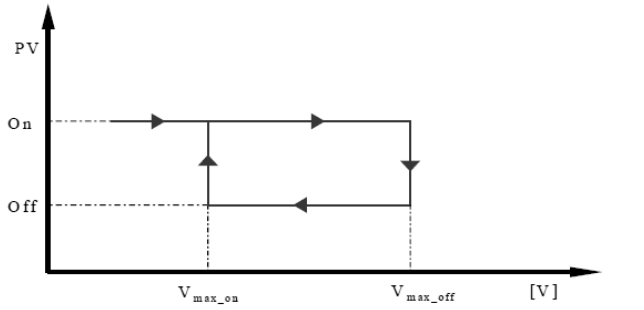
\includegraphics[width=0.4\textwidth]{controllerover}
%\centering
%\caption{Operating principle of an overcharge protector (Source: \cite{Hansen})}
%\label{fig:controllerover}
%\end{figure}
%
In order to protect the battery against excessive discharge, the load is disconnected when the terminal voltage falls below a certain threshold $V_{min \textunderscore off}$ and when the current required by the load is larger than the current delivered by the PV arrays~\cite{Hansen}. The load is reconnected to the system, when the terminal voltage is above a certain value $V_{min \textunderscore on}$.
%, using a switch with a hysteresis cycle, as shown in Fig. \ref{fig:controllerdisc}. 
%
%\begin{figure}[h]
%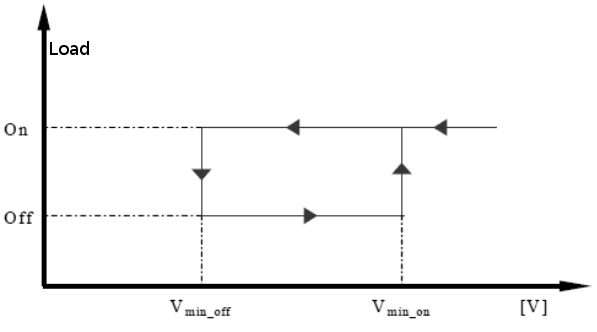
\includegraphics[width=0.4\textwidth]{controllerdisc}
%\centering
%\caption{Operating principle of a discharge protector (Source: \cite{Hansen})}
%\label{fig:controllerdisc}
%\end{figure}
%
%According to \cite{Lorenzo}, the switches may either be electromechanical (relay, contactors, etc.) or solid state (bipolar transistors, MOSFET's, etc.). 
%
The steps in the modeling of the controller process are summarized in Table~\ref{table:controller}.

\begin{table}[!t]
%% increase table row spacing, adjust to taste
\renewcommand{\arraystretch}{1.3}
% if using array.sty, it might be a good idea to tweak the value of
% \extrarowheight as needed to properly center the text within the cells
\caption{Summary of the controller process (Source:~\cite{Hansen})}
\label{table:controller}
\centering
%% Some packages, such as MDW tools, offer better commands for making tables
%% than the plain LaTeX2e tabular which is used here.
\begin{tabular}{c | c | c }
\hline
\hline
Step  & Constraint & Command\\
\hline
\hline
(1) & \makecell{If $V > V_{max \textunderscore off}$ \\and $I_{load} < I_{pv}$} & \makecell{Disconnect PV array \\from the system}\\
\hline
(2) & \makecell{If command (1) is \\done and $V < V_{max \textunderscore on}$} & \makecell{Reconnect PV array \\to the system}\\
\hline
(3) & \makecell{If $V < V_{min \textunderscore off}$ and \\ $I_{load} > I_{pv}$} & \makecell{Disconnect the load \\from the system}\\
\hline
(4) & \makecell{If command (3) is \\ done and $V > V_{min \textunderscore on}$} & \makecell{Reconnect the load \\to the system}\\
\hline
\hline
\end{tabular}
\end{table}

%Regarding the DC-DC converter, the most basic idea is that the power is converted while altering the current and voltage. 
%
%As shown in \cite{Abdulateef}, the DC-DC converter is used to increase the efficiency of the PV system by matching the voltage generated by PV array to the voltage required by the load. 
The output power ($ P_{out} $) of DC-DC converter is given by Eq.~\eqref{eq:poutcont} as
\begin{equation}
\label{eq:poutcont}
P_{in} = P_{out}.
\end{equation}

Assuming that the efficiency of the controller ($ \eta_{c} $) is a manufacturer's data, from Eq.~\eqref{eq:poutcont} we compute Eq.~\eqref{eq:potcont} as
\begin{equation}
\label{eq:potcont}
V_{in} I_{in} \eta_{c} = V_{out} I_{out},
\end{equation}

\noindent where $ V_{in} $ is the voltage across the PV array, $ I_{in} $ is the output current of PV array, $ V_{out}=V_{b}=V_{system} $ is the  DC bus voltage, and $ I_{out} $ is the output current from the converter.

%The output voltage is related to the input voltage as a function of duty cycle of the switch (\cite{Abdulateef}). 
% 
%A DC-DC converter can either be step-up (Boost), step-down (Buck), or both increase and decrease (Buck-Boost) the voltage, as defined by \cite{Mahanta}. In addition, there is the Cuk converter, which is a Buck-Boost converter with an inverting topology \cite{Catherine}. 
%
%For the Cuk converter, the relationship is expressed by \ref{eq:voutvin} as show in \cite{Abdulateef}.
%
%\begin{equation}
%\label{eq:voutvin}
%\dfrac{V_{out}}{V_{in}} = \dfrac{D}{D-1}
%\end{equation}
%
%Where $D$ is the duty cycle or ratio of the circuit converter, i.e., it is defined as the ratio of the on time of the switch to the total switching period.
% 
%The DC/DC converter should always operate in the MPPT to maximize the PV array efficiency and consequently increase the efficiency of the PV system, as defined in \cite{Yatimi}.
%  
%Various types of MPPT schemes are proposed by researchers, namely open circuit, short circuit, perturb and observe (P\& O)/hill climbing, incremental conductance, and so forth, as shown by \cite{Haque}.
% 
%As the MPPT definition and the equations to get the maximum power from the PV panels was described at the end of the PV panel modeling, the important here is to notice that the Equation \ref{eq:voutvin} defines the relationship between the input signal, the efficiency of the controller and the output power.
 
One more time, some steps must be done to check the sizing project of the controller, prior the verification phase. Initially, the controller must meet the voltage requirement of the PV system, as described by Eq.~\eqref{eq:vcvsystem}: 
\begin{equation}
\label{eq:vcvsystem}
V_{c} = V_{system}.
\end{equation}

Following, the short circuit reference information from the manufacturer's solar panel must be corrected to the cell temperature, as described by Eq.~\eqref{eq:iscamb}:
%
\begin{equation}
\label{eq:iscamb}
I_{sc,amb} = I_{sc,ref} \times \left[ 1 + \eta_{I} \times (T-25) \right]. 
\end{equation}

The controller must meet the maximum current from the PV array given by \eqref{eq:icmin} and \eqref{eq:icicmin}.
\begin{equation}
\label{eq:icmin}
I_{c,min} = I_{sc,amb} \times N_{PP}.
\end{equation}

\begin{equation}
\label{eq:icicmin}
I_{c} \geq I_{c,min}.
\end{equation}

%The number of controllers required for the stand-alone PV system, as defined by \cite{Yatimi}, is calculated using Equation \ref{eq:numberofcmin}. In addition, the final sizing check is did by Equation \ref{eq:numberofc}, who validate the number of controllers adopted.
%\begin{multline}
%\label{eq:numberofcmin}
%number_{controllers} = \dfrac{Total \, max \, power \, of \, PV}{Controller \, max \, power} = \\ \dfrac{P_{m,ref} \times N_{TP}}{V_{system} \times I_{controller,max}}
%\end{multline}
%
%\begin{equation}
%\label{eq:numberofc}
%N_{controller} \geq number_{controllers}
%\end{equation}
%
%\subsection{Joint work: charge controller and batteries}
%When batteries are charged, they go through three main different states - bulk, absorption and float, with impact to the inverter and to power supplied to the house.
%, and it is necessary to understand those three states in order to comprehend the joint work of the controller with the battery. With impact to the inverter and to power supplied to the house. 
%
%All the explanation at this section is related to $SOC$ and to the voltage at the DC-bus (controller output, which will be bigger than $V_{system}$) where the batteries are connected, all ruled by the charge controller. Moreover, it is important to mention that smart chargers, the most usual nowadays, will detect voltage and resistance from the battery prior to charging.
%
%Bulk - is the first stage of charging. Bulk begins when the sun comes out.
%, or other source of electrical generation is turned on. 
%This stage occurs when the batteries are at a lower $SOC$, generally anything not smaller than $75\%$ to $80\%$ (defined during system sizing). This stage is typically where the highest voltage and current the charger is rated for will actually be used. The bulk stage basically allows the PV panel to put as much current into the batteries as possible. For a typical 12 V battery, the charging voltage going into a battery will reach 14.16 V to 14.40 V at this stage, and there is no risk of overcharging in this stage because the battery hasn't even reached full yet.
%
%Absorption - once the batteries reach the programmed absorb voltage, usually somewhere between 14.16 and 14.40 V, the batteries will go into the absorption stage. Typically, when a battery reaches this stage its $SOC$ is around $85-95\%$. During this stage, the batteries are kept at the programmed voltage, and the current going into the batteries reduces as the batteries become more full. The absorption stage ends after the programmed time is reached or the number of Ampere going into the battery falls below a preset number. The lower current going into the battery safely brings up the charge on the battery without overheating it. 
%Usually, this stage takes more time than the bulk stage.
%
%Float - upon the completion of the absorption stage, the charge controller will  drop down the voltage and maintain at a steady 13.20 V to 13.38 V (manufacturer's defined value), which is the maximum voltage that a 12 V battery can hold, and begin the float stage. The float stage brings the battery all the way through and maintains $SOC$ at $100\%$. The current will also decrease to a point where it's considered just a pulse. It's essentially the float stage where there is charge going into the battery at all times, but only at a safe rate to ensure a full state of charge and nothing more. 
%Most smart chargers do not turn off at this point, however it is completely safe to leave a battery in float mode for months to even years at a time.
%
%Battery charging technology relies on smart micro-controlled devices. Therefore it is extremely important that the program settings for the charge controller or inverter/charger are correct, and the list includes the bulk and absorption values. 
%This will help preserve and extend the battery life. There are always default settings to the equipment, set by software, however those settings are not $100\%$ correct because there are difference among models of equipment and among manufacturer's. The ideal is to read the data-sheet from the manufacturers and perform a manual adjust.
%
%There are the possibility to combine batteries in a bank, with parallel and series connections, all depending the sizing of the project:
%
%\begin{itemize}
%\item Batteries connected in parallel are seen by the controller as one large battery of the combined Ah capacity of all the batteries. For example, two 12 V and 220 Ah batteries in parallel are seen as one 12 V and 440 Ah battery;
%\item In the other hand, although the batteries connected in series are also seen as a single battery, the result is different: two 12 V and 220 Ah batteries in series are seen as one 24 V and 220 Ah battery;
%\item In addition, a mixed bank arrangement can be useful: a bank with two 12 V and 220 Ah batteries in series connected in parallel with a similar arrange will produce an equivalent battery of 24 V and 440 Ah.
%\end{itemize}
%-----------------------------------------------
\subsection{The inverter model}
%-----------------------------------------------
%As shown by \cite{Mellit}, the PV arrays produce DC and therefore when the PV system contains an AC load, a DC/AC conversion is required. 
%An inverter is a converter, where the power flows from DC to AC side, i.e., having a DC voltage as input; it produces AC voltage, as output. 
The role of the inverter is to keep the voltage constant on the AC side, i.e., at the rated voltage, % (127 V or 220 V, for example), 
and to convert the input power $ P_{in} $ into the output power $ P_{out} $ with the best possible efficiency $ \eta_{i} $ as described by Eq.~\eqref{eq:efficinv} \cite{Hansen}:
%
%The inverter is characterized by a power dependent efficiency $ \eta_{i} $ as shown by (\ref{eq:efficinv}) \cite{Hansen}.
\begin{equation}
\label{eq:efficinv}
\eta_{i} = \dfrac{P_{out}}{P_{in}} = \dfrac{V_{AC} I_{AC} cos\varphi}{V_{DC}I_{DC}},
\end{equation}

\noindent where $ I_{DC} $ is the current required by the inverter from the DC source to be able to keep the rated voltage on the AC side, $ V_{DC} $ is the input voltage to the inverter delivered by the DC source (PV panel or battery),  $ V_{AC}  $ and $ I_{AC} $ are the output voltage and current, respectively, and $ cos \varphi $ can be obtained from the inverter's data-sheet.

%Therefore, with this equation it is possible to simulate the output power of the inverter, based on information from the inverter's data-sheet and from the DC module or the PV panel that feed the inverter (which are obtained by this study model). 
%
The sizing project check of the inverter is carried out by means of three equations. Eq.~\eqref{eq:vindc} ensures that the input voltage of the controller meets the system voltage. Eq.~\eqref{eq:voutac} ensures that the output voltage of the controller meets the AC voltage of the load. Finally, Eq.~\eqref{eq:invcheck} ensures that the controller can support the total demand of the load and the surge power.
%
\begin{equation}
\label{eq:vindc} 
V_{in}DC = V_{system}.
\end{equation}
%
\begin{equation}
\label{eq:voutac} 
V_{out}AC = V_{AC}.
\end{equation}
%
\begin{equation}
\label{eq:invcheck} 
\left[ (Demand \leq P_{AC,ref}) \, and \, (P_{surge} \leq MAX_{AC,ref}) \right].
\end{equation}

%--------------------------------------------------
\section{Automated Verification Using Model Checking}
\label{sec:AutomatedVerification}
%--------------------------------------------------
%It is necessary to keep in mind that 
Validation is the process of determining whether a design meets the user requirements, whereas verification is the process of determining whether a design meets a set of requirements, specifications, and regulations~\cite{ClarkeHV18}. If the requirements, specifications, and regulations are given in a formal language, then it may be possible to automate the verification process, thus resulting in a process known as \textit{formal verification}. Verification may form part of a validation process.
%, but in general, validation cannot be formalized because it relates a system design to intent.  
While simulation and testing explore some of the possible behaviors and scenarios of the system, leaving open the question of whether the unexplored trajectories may contain a flaw, formal verification conducts an exhaustive exploration of all possible behaviors. Thus, when a design is pronounced correct by a formal verification method, it implies that all behaviors have been explored, and the questions of adequate coverage or a missed behavior becomes irrelevant \cite{Clarke2012}.
%Simulation may also be used for validation, but it is more problematic for verification.
%In order to use simulation for verification, it is necessary to ensure adequate coverage of operating conditions, scenarios, and system inputs. Testing can also be used for validation, however it is not feasible to cover all the aspects of the design space, and some times the real system must be used instead of a computing model.
 %

Formal verification is a systematic approach that applies mathematical reasoning to obtain guarantees about the correctness of a system \cite{Forejt2011}; one successful method in this domain is model checking \cite{Clarke2012}.
 % 
%Model checking is an automatic verification technique, as defined by \cite{ClarkeHV18}. Model checking was originally developed reasoned about finite state of concurrent systems, nowadays is mainly used to hardware and software verification, but can be applied to any kind of system. 
%
The process of model checking can be split into three main components: modeling, specification, and verification method. In modeling, a model (normally mathematical) of the system is created; in specification, normally a list of properties to be satisfied by the system is established, i.e., the requirements, normally  expressed in a temporal logic form (e.g., CTL or LTL).
%
%\begin{itemize}
%\item In modeling, a model (normally mathematical) of the system is created; 
%\item In specification, normally a list of properties to be satisfied by the system is established, i.e., the requirements, as reliability to performance for example. \item Normally is expressed in temporal logic form ($CTL$); 
%\item The model checking is the verification method itself. 
%\end{itemize}
%
The model checking algorithm can be described as \cite{ClarkeHV18}:  
%
\begin{itemize}
\item Given the model $M$ and a CTL (or LTL) formula $ \phi $ as input;  
\item Model checking algorithm provides all the states of model $ M $ which satisfies $ \phi $;  
\item It returns \textit{YES} if $ \phi $ is \textit{TRUE}, or returns \textit{NO} if $ \phi $ is \textit{FALSE}.  
\end{itemize}
Specifically for the \textit{FALSE} verification result, the algorithm returns a \textit{counterexample} (i.e., a sequence of states that leads to a property violation), which is useful as diagnostic of the system to discover in which situation the model is violated; this is the most important advantage of the use of model checking~\cite{ClarkeHV18}. 
%Among the other advantages can be listed: there is no need of proofs (the algorithm is not a deductive procedure), there is no problem with partial specifications of the system, logics can easily express many concurrency properties, is fast (compared to other rigorous methods such as interactive theorem proving). 
%
%The model checking problem can be defined as \cite{ClarkeHV18}: 
%
%\begin{itemize}
%\item Let $M$ be a Kripke structure (i.e., state transition graph);
%\item $f$ be the specification in temporal logic (a formula);
%\item Find all states $s$ of $M$ such that $M , s \models f$
%\end{itemize}
%
%Fig. \ref{fig:modelcheckstruc} shows the structure of a 
%In a typical model checking system, a preprocessor extracts a state transition graph from a system (program or circuit).
%
%\begin{figure}[h]
%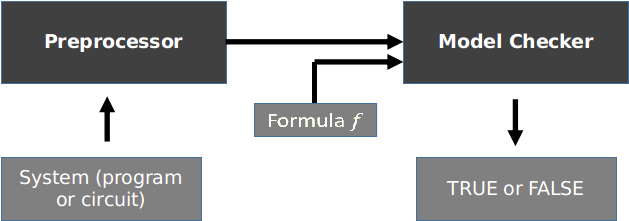
\includegraphics[width=0.4\textwidth]{modelcheckstruc}
%\centering
%\caption{Model Checker structure (Source: \cite{ClarkeHV18})}
%\label{fig:modelcheckstruc}
%\end{figure}
%
%Here it is worth to mention that the term "model" is not the meaning taken from the dictionary. The problem is not dealing with an abstraction of the actual system under study. 
%
Fig.~\ref{fig:systemverif} shows the process to convert a real PV system to a model to be verified by a model checking procedure. % \textcolor{red}{Please try to adapt this figure to our context. How can it be applied to verify PV?}. 

\begin{figure}[h]
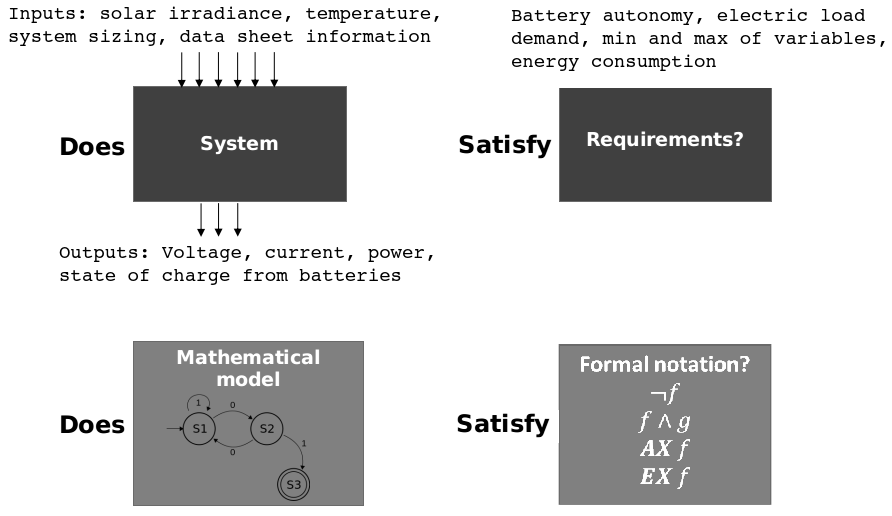
\includegraphics[width=0.5\textwidth]{systemverif2}
\centering
\caption{From real system verification to model checking (adapted from \cite{ClarkeHV18}).}
\label{fig:systemverif}
\end{figure}

However, there is a main disadvantage of model checking: the state explosion problem. In order to tackle this problem, many different techniques were developed in the last decades. One of the first major advances was symbolic model checking with binary decision diagrams (BDDs). In this approach, a set of states is represented by a BDD instead of by listing each state individually, which is often exponentially smaller in practice.
% Another major advance is the partial order reduction, which exploits the independence of actions in a system with asynchronous composition of processes \textcolor{red}{add citation here}. A third major advance is counterexample-guided abstraction refinement, which adaptively tries to find an appropriate level of refinement, not burdened with irrelevant detail that slows down verification \cite{Clarke2012}. 
%
Another promising approach to overcome state explosion problem is Bounded Model Checking (BMC)~\cite{DBLP:conf/tacas/BiereCCZ99}. BMC is a method that checks a model up to a given path in the path length. BMC algorithms traverse a finite state machine for a fixed number of steps, $ k $, and checks whether a property violation occurs with this bound. It uses Boolean Satisfiability (SAT) or Satisfiability Module Theories (SMT) solvers to check the generated formula from BMC. 

SAT problem is a problem of determining whether there are certain conditions or interpretations that satisfy a given Boolean expression \cite{ClarkeHV18}. 
SMT decides the satisfiability of a fragment of first-order formulae using a combination of different background theories and thus generalizes SAT by supporting uninterpreted functions, linear and non-linear arithmetic, bit-vectors, tuples, arrays, and other decidable first-order theories~\cite{ClarkeHV18}.
The SAT or SMT solvers search the model for conditions (value of variables) that make the formula satisfiable. If a SAT or SMT solver finds a substitution for the formula/function then the substitute induces a counterexample and is said to be \textit{satisfiable}, i.e., it is satisfiable \textit{iff} the verified system contains errors.  
%
%CBMC is considering the best-known model verification tool to validate code in ANSI-C and C++ \cite{Kroening}. 
%
%\textcolor{red}{ESBMC does not use CBMC as its main frontend. Please take a look at this paper and cite it: https://ssvlab.github.io/lucasccordeiro/papers/ase2018.pdf. I would also suggest to remove the above sentence.}
%
ESBMC is one of the most representatives bounded model checkers for embedded C/C++ software based on SMT solvers~\cite{esbmc2018}. %, which can use CBMC as front-end.
%The use of SMT, instead of Boolean Satisfiability SAT from the original BMC, 
ESBMC comes as an alternative to overcome limitations of the system modeling, especially considering that the system complexity is increasing and SMT has richer theories than SAT to represent models. 

%--------------------------------------
\subsection{ESBMC}
%--------------------------------------
ESBMC (or Efficient SMT-based Bounded Model Checker) is an open source, permissively licensed (Apache 2), cross platform bounded model checking for C and C++ programs~\cite{esbmc2018}, which supports the verification of LTL properties with bounded traces~\cite{DBLP:journals/sosym/MorseCN015}. 
%
ESBMC's verification flow can be summarized in three stages: (i) a front-end that can read and compile C/C++ code, where the formal specification of the system to be verified is first handled; (ii) preprocessing steps to deal with the representation of the code, control flow and unwinding of loops, and the model simplification, thereby aiming to reduce the verification effort; and finally (iii) the SMT solving stage, where all the constraints and properties of the system to be verified are encoded into SMT and checked for satisfiability.
%
%%The efficient SMT based model checker, is a software verification tool for C and C++ code bases. 
%
%%%%%%%%%%%%%%%%%%%%%%%%%%%%%%%%%%%%%%%%%%%%%%%%%%%%%%%%%
%%%%%%%%%%%%%%%%%%%%%%%%%%%%%%%%%%%%%%%%%%%%%%%%%%%%%%%%%
%Fig. \ref{fig:esbmcarch} shows the tool architecture. 
%
%\begin{figure}[h]
%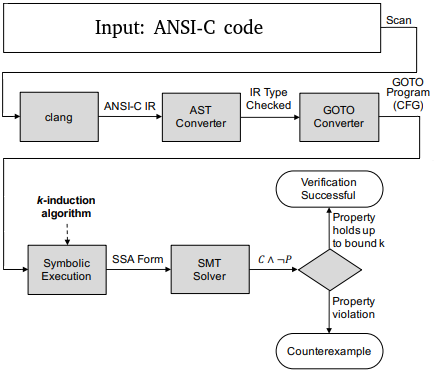
\includegraphics[width=0.4\textwidth]{ESBMCarch4}
%\centering
%\caption{ESBMC architecture (adapted from \cite{esbmc2018}).}
%\label{fig:esbmcarch}
%\end{figure}
%ESBMC uses clang as front-end, a state-of-the-art compiler suite for C/C++/ObjectiveC/ObjectiveC++ widely used in industry \cite{esbmc2018}. % and generate an Abstract Syntax Tree (AST). %%%%%One legacy CBMC-based front-end that supports both C and C++ and a new clang-based front-end that currently only supports C. The data types and bit vectors are created in the front-end when parsing the code. 
%%%%%%%Regardless of the chosen front-end, 
%The output is an AST (tree representation of the abstract syntactic structure of source code written in a programming language) that will be used by the GOTO converter to generate a GOTO program, which has simplified control flow and is suitable for bounded unwinding. The next step is the symbolic execution, when the GOTO program is executed (unrolling loops up to the bound $ k $) and converted to Static Single Assignments (SSA) form. SSA form enables the simplification of algorithms and reduction of computational complexity. %%%%%%%%%, where each variable is a target of exactly one assignment statement in the program text. 
%The feature called k-induction at Fig. \ref{fig:esbmcarch} allows the model checker to find a property violation or even to prove (partial) correctness without fully unwinding loops. 
%%
%%%%%%%During the symbolic execution, ESBMC aggressively tries to simplify the program \cite{Ramalho}; it propagates all constants and solves any assertions that can be statically determined. This is an important step for the verification, since ESBMC can fully verify programs without calling a solver, if the inputs are deterministic. That characteristic is useful at this work to perform the sizing check of the PV system project. 
%Following, the SSA expressions are then encoded using the chosen SMT solver supported by ESBMC. At this paper, it was used the Z3 solver \cite{DeMoura}.
%%%%%: Boolector (default) \cite{Brummayer}, Z3 \cite{DeMoura}, MathSAT \cite{Cimatti}, Yices \cite{Dutertre} and CVC4 \cite{Barrett}. 
%
%Finally, the system attempting to determine whether a formula, which is the disjunction of all possible errors, can be satisfied. 
If the SMT formula is shown to be satisfiable (SAT), a counterexample is presented; otherwise, the formula is unsatisfiable (UNSAT), i.e., there are no errors up to the given unwinding bound. 

% incremental ESBMC text here
ESBMC exploits the standardized input language of SMT solvers (SMT-LIB\footnote{http://smtlib.cs.uiowa.edu/} logic format) to make use of a resource called \textit{assertion stack}. An assertion, in SMT solvers, is a constraint over the variables in a formula that must hold if the formula is satisfiable~\cite{Morse2015}. New assertions can be added to or old assertions removed from this stack, depending on the evaluated value of variables. This enables ESBMC, and the respective solver, to learn from previous checks, optimizing the search procedure and potentially eliminating a large amount of formula state space to be searched, because it solves and disregards data during the process, incrementally. This technique is called ``incremental SMT''~\cite{DBLP:journals/fac/SchrammelKBMTB17} and allows us to reduce the memory overhead, mainly when the verified system is complex and the computing platform does not have large amount of memory to deal with all the design space state.

%
%%%%%%%%%%%%%%%%%%%%%%%%%%%%%%%%%%%%%%%%%%%%%%%%%%%%%%%%%%%%%%%%%%%%%%%%%5%
%%%%%ESBMC can be invoked through the command-line interface or configured through the Eclipse plug-in. Specific problems and the solver can be selected that way. 
%
%ESBMC aims to support all of ISO/IEC 9899:2017 C programming language standard, and detects errors in software by simulating a finite prefix of the program execution with all possible inputs. Classes of problems that can be detected include: user specified assertion failures, out of bounds array access, illegal pointer dereferences, double-free of malloc'd memory, misaligned memory access; integer overflows, divide by zero, memory leaks, concurrent software, deadlock, and data races (i.e. competing writes). 
 
%\subsection{Cyber-physical systems x Energy x ESBMC}
%According \cite{UC}, cyber-physical systems (CPS) are integrations of computation, networking, and physical processes. Embedded computers and networks monitor and control the physical processes, with feedback loops where physical processes affect computations and vice-versa. The economic and societal potential of such systems is vastly greater than what has been realized, and major investments are being made worldwide to develop the technology. The technology builds on the discipline of embedded systems (computers and software embedded in devices) whose principle mission is not computation, such as cars, toys, medical devices, and scientific instruments. CPS integrates the dynamics of the physical processes with those of the software and networking, providing abstractions and modeling, design, and analysis techniques for the integrated whole. 
%
%Energy production, distribution, and optimization are all CPS problems, mas mentioned in \cite{UC}. For example, the smart grid combines multiple electric power production plants with a multiplicity of loads using dynamic load balancing and dynamic pricing with demand-response strategies. Smart buildings integrate sensors into control systems for lighting, HVAC (heating, ventilation, and air conditioning), and safety (as fire monitoring and evacuation). 
%
%Therefore, in the context of this proposal, a cyber-physical system, specifically a solar photovoltaic system, will be mathematically modeled. Then a model checking will be performed to do a verification of the project in order to guarantee that the design of a stand-alone PV solution will meet the requirements, specifications and regulations. 
%
%As described in \cite{Alur}, in program verification, it is aimed to check if a program satisfies its logical specification. Contemporary verification tools vary widely in terms of source languages, verification methodology, and the degree of automation, but they all rely on repeatedly invoking an SMT solver. This work tracks the same path. 
%
%----------------------------------------
\section{Model Checking Stand-alone Solar Photovoltaic Systems }
\label{sec:Methodology}
%----------------------------------------
%
%Fig. \ref{fig:statetransition} shows the state diagram for the proposed tool. 
%
%\begin{figure}[h]
%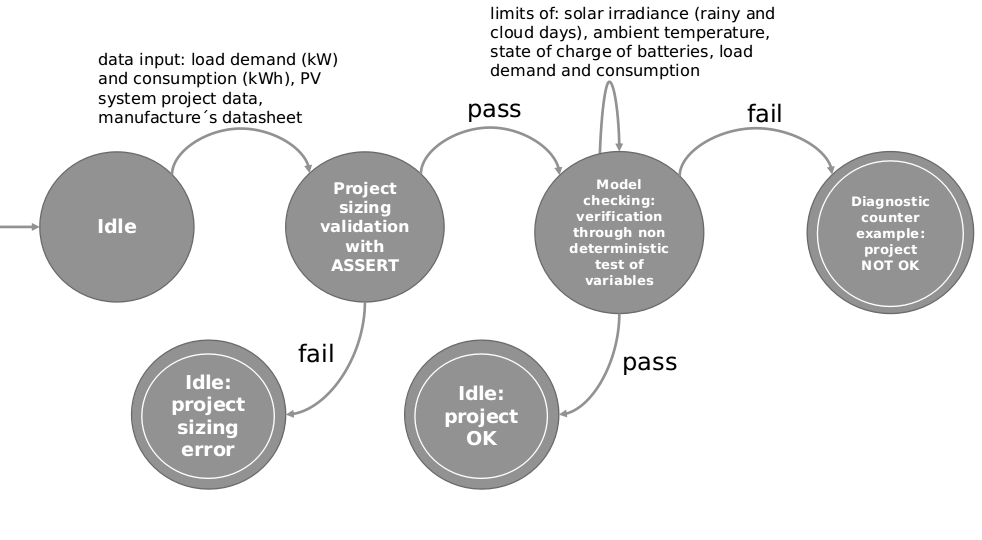
\includegraphics[width=0.5\textwidth]{statetransition}
%\centering
%\caption{State transition diagram to the proposed automated verification.}
%\label{fig:statetransition}
%\end{figure}
%
%It is worth mentioning that the steps described here are carried out shortly after the design of the solar photovoltaic system, as soon as the equipment and equipment specifications are defined; before buying and deploying them, as a way to ensure that the project will not fail. 
%
The flowchart of the proposed automated verification method is illustrated in Fig.~\ref{fig:flowchartgeneral}. 
In Step 1, the PV input data (e.g., load power demand and load energy consumption) and the formulas to check the sizing project, the mathematical model, the limits of the weather non-deterministic variables, are all written as an ANSI-C code~\cite{ANSI2018}. In Step 2, the sizing check of the PV system takes place to make sure that the components were selected in accordance with recognized design standards \cite{Pinho}.
\begin{figure}[h]
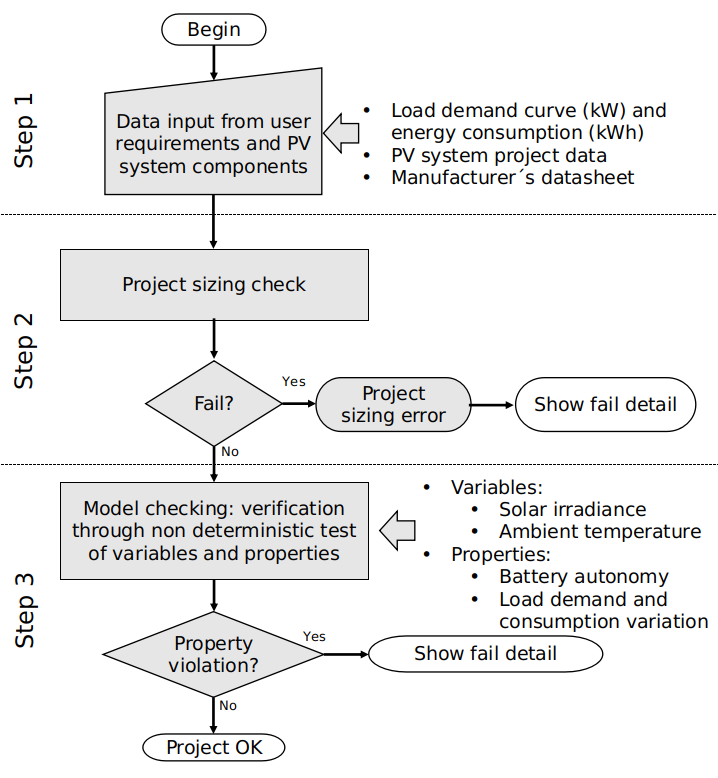
\includegraphics[width=0.4\textwidth]{flowchart_verification4.png}
\centering
\caption{Flowchart of the proposed automated verification of PV systems.}
\label{fig:flowchartgeneral}
\end{figure}
%
In Step 3, weather variables (e.g., solar irradiance and ambient temperature) will be systematically explored by our verification engine based on maximum and minimum values from the site, where the PV system will be deployed. As a consequence, all the formulas of the employed mathematical models will also be updated. In addition, depending on one of the desired properties of the system, as autonomy of the batteries, the offer of the energy, or even the power supply from the system to check, whether it is not accomplished (said satisfied), ESBMC accuses a failure, and the diagnostic counterexample shows in which condition the property violation (system fail) happened. 
%; as the  state of charge of the batteries, load demand of power and the load consumption of energy if defined by the code
% (as reliability, performance, or safety)

%
%\textcolor{red}{In the following paragraph you should related the output of our verification engine with the description of the BMC SAT or UNSAR given above. For example, what does a failure mean? is it SAT?}
In a nutshell, ESBMC will process the C code with constraints %($C$) 
and properties %($P$) 
from the PV system that were provided by the user, and the tool will verify automatically if the PV system requirements are met. If the return is a failure (i.e., SAT), then the tool details the condition of violation, i.e., the state of each variable related to the system. That information can be used as a feedback to improve the PV system project. However, if the verification succeeds (i.e., UNSAT), there is no failure, therefore the PV system will present its intended behavior up the bound $k$, i.e., it does not give any guarantee that there is no error in bound $k+1$ unless some induction method is employed~\cite{DBLP:journals/sttt/GadelhaIC17}.
%
%
%---------------------------------------------------------------------
% \subsection{The case studies and the Algorithm}
%---------------------------------------------------------------------
%
% 
%and as backup at night 
%
%The 700 W system: 3 x 325 W PV panels connected in series, controller of 150 V/35 A with a DC-bus of 24 V, 4 x 220 Ah batteries (2 in series and 2 in parallel arrangement), and inverter of 700 W. 
%
%And the 1,200 W PV system: 4 x 325 W connected in series PV panels, with controller of 150 V/35 A  in a DC-bus of 48 V, 4 batteries of 120 Ah connected in series, and a 1,200 W inverter.
%
%As demonstrated at this work, the performance of the system is highly dependent of solar irradiance and temperature, that are specific of the deployed local (latitude and longitude). 

Algorithm~\ref{alg:verification-algorithm} describes the pseudocode used to perform the automated verification. Line 1 indicates a function call that performs the size checking of the entire PV system: using Equations \eqref{eq:NTPmin}, \eqref{eq:NTP}, \eqref{eq:NPSmin}, \eqref{eq:NPS}, \eqref{eq:NPP}, and \eqref{eq:NPPmin} to verify the PV panel; using \eqref{eq:Cbank}, \eqref{eq:Nbtotal}, and \eqref{eq:batcheck} to verify the batteries; using \eqref{eq:vcvsystem}, \eqref{eq:icmin}, and \eqref{eq:icicmin} to verify the charge controller; and using \eqref{eq:vindc}, \eqref{eq:voutac}, and \eqref{eq:invcheck} to verify the inverter. The verification is performed by the standard \textit{assert} macro from the ANSI-C programming language to each equation. The argument to the \textit{assert} statement must be \textit{true} if the system specification is met; otherwise, the program aborts and prints an error message indicating a property violation. If there is no property violation, then the verification algorithm continues and the batteries are assumed to have SOC of 80\% (Line 5).

%At both case studies, it was considered 21 years of historic data from Manaus. 
%According with X and Y, t
Information related to average temperature ($T$) and solar irradiance ($G$), maximum and minimum annual, are given to the algorithm in Lines 7 to 10 using the feature of non-deterministic variables from ESBMC to explore all possible states and the \textit{assume} macro to limit the non-deterministic values considering a given range. 
%and irradiance varies from 0 W/m$^{2}$ to 852 W/m$^{2}$ (with minimum of 274 W/m$^{2}$ during the daytime, when there is sunlight). 
%there is PV generation only between 8:00 h and 16:00 h every day, 
%with zero electric energy generation from 18:00 h to 6:00 h of the next day; and with insignificant generation from 6:00 h to 8:00 h, and from 16:00 h to 18:00 h of the same day. 
In order to reduce the computational effort of the algorithm,
% caused by the state explosion inherent of the technique, 
every 24h-day was considered as a time-step of 1 hour, and it was split into two parts: (a) one where it is possible to occur PV generation, during daylight, with a duration in hours depending on each site (but dependent of the sun and weather conditions); and (b) one that includes all the remaining day (without any PV generation). Therefore, the proposed methodology depends on specific data about the solar irradiation levels to define the average amount of hours of PV generation.

After that, the model from PV generator is used in the function call of Line 11, to produce the voltage and current considering the states of $G$ and $T$. Following, related to every hour considered, the conditional \textit{if-else-endif} statements from Lines 12, 17, 23 and 28, will perform the charge or discharge of batteries according to the value of different variables: if there is PV generation (which depends on $G$ and $T$), the updated state of charge from batteries, the house's load and the set-up information of the PV system.

Next, representing the time of the day where is not possible PV generation anymore, starting at Line 31, the algorithm will only discharge the batteries (using the 1 hour step) until a new charging process (at the next day) to start. Specific macro commands, the \textit{assert} at Lines 27 and 35, it will check the state of charge from batteries, and it will violate the property if its level reach the minimum that represents a discharged battery. And, therefore, the PV system is not able to supply energy to the house. In the other hand, if the automated tool do not fail, then the code is finalized with success and the PV system do not need improvements or corrections.
%
%\textcolor{red}{this sentence is unclear... After this process is started the battery autonomy verification, from line 31}. \textcolor{red}{this sentence is unclear... Based on the fact that won't be PV generation after a given time of the day, the algorithm will only discharge the batteries until a new charging process (at the next day) to start.} \textcolor{red}{what do you mean by The formal verification is guaranteed?...  The formal verification is guaranteed by  macro to specific variables of the model, according lines 27 and 35.}
% and the non-deterministic variables $G$ and $T$ are considered during the formal verification of the system, otherwise, during the other two periods, there is no PV generation and just the power consumption from the backup batteries. 
%Within this 8h-period, $G$ and $T$ are automated verified with different values every one hour.
%, and change their value every 1 h according with the algorithm created using the technique.
 \begin{algorithm}
 \caption{Algorithm to perform automated verification}
 \begin{algorithmic}[1]
 \renewcommand{\algorithmicrequire}{\textbf{Input:}}
 \renewcommand{\algorithmicensure}{\textbf{Output:}}
  \STATE Perform project sizing verification( )
  \IF {(FAIL verification)} 
  \STATE exit ("Project sizing error")  
  \ENDIF
  \STATE $SOC \leftarrow 80\%$ \\
  \COMMENT {Starting with the PV generation time}
 \\ \textit{LOOP Process}
  \FOR {$h = 1$ to $Hours \, of \, PV \, generation$}
  \STATE $G \leftarrow nondet \textunderscore uint(\,)$ \COMMENT {$G$ is non-deterministic variable}
  \STATE $T \leftarrow nondet \textunderscore uint(\,)$ \COMMENT {$T$ is non-deterministic variable}
  \STATE assume ($Gmin \leq G \leq Gmax$) \COMMENT {restricting $G$ values}
  \STATE assume ($Tmin \leq T \leq Tmax$) \COMMENT {restricting $T$ values}
  \STATE $Imax, Vmax \leftarrow PVgenerationMODEL (G,T)$ 
  \\
  \COMMENT {Now, testing if battery is empty:}
  \IF {($SOC \leq SOC_{limit}$)} 
    \STATE assert (PV panel is generating energy?) \COMMENT {FAIL if not}
    \STATE $house \leftarrow energy \, from \, PV \, panels$
    \STATE $battery \leftarrow energy \, from \, PV \, panels$ 
    \STATE $SOC \leftarrow SOC + 1\,h\, charge$
  \ELSIF {($PV \, Array  \geq Vbulk$)}
  	\STATE depending on $SOC$, Battery enter in absorp. or float.
	\STATE adequate the voltage at DC-bus (PV panel feed bus)
    \STATE $house \leftarrow energy \, from \, PV \, panels$
    \STATE $battery \leftarrow energy \, from \, PV \, panels$ 
    \STATE $SOC \leftarrow SOC + 1\,h\, charge$
  \ELSE
  	\STATE Adequate the voltage of DC-bus (battery feed bus)
	\STATE $house \leftarrow energy \, from \, batteries$
    \STATE $SOC \leftarrow SOC - 1\,h\, discharge$
    \STATE assert ($SOC \geq SOC_{limit}$)
    \\
    \COMMENT {this ELSE: batteries $\geq SOC_{limit}$ but panels are off}	  
  \ENDIF
  \STATE $h \leftarrow (h+1)$
  \ENDFOR
 \\ \textit{Start of battery autonomy verification:}
%%  initialization\;
\STATE $AutonomyCount \leftarrow 1$
 \WHILE {$AutonomyCount \leq autonomy$}
  %%\FOR {$Autonomy = 1$ to $auton$}

  \STATE $SOC \leftarrow SOC - ( 24 - Hours \, of \, PV \, generation)\,h\, discharge$
  \STATE $AutonomyCount \leftarrow ( 24 - Hours \, of \, PV \, generation)$
  \\  
    \COMMENT {autonomy verification during discharge period}
  \\
  \STATE assert ($SOC \geq SOC_{limit}$)  
  \\
  \COMMENT {Perform similar \textbf{for}-LOOP as defined in line 6}
  %%\ENDFOR
  \ENDWHILE
 \RETURN $(\,)$ 
 \end{algorithmic} 
 \label{alg:verification-algorithm}
 \end{algorithm}
%There are two premises considering the algorithm: (1) is considered a $SOC$ of 80\% at 8:00 h, and is made the automated evaluation from 8:00 h to 16:00 h, but without to account the battery autonomy (just considering charge and discharge process based on solar irradiation, load and battery charge), but after 16:00h is started the verification for the next hours when there is not solar photovoltaic generation. The process goes on until to verify all the autonomy demanded from the batteries; (2) there is an array, declared at the beginning of the C code, that defines the power demand/consumption at each hour of the day (aka load curve). Those are the same data used during the sizing of the project and ensure to consider the total energy (per day) supplied to the house during the verification. 
%
%If the verification founds a situation where the electrical demand of the house is not met, then the algorithm presents a counterexample of this combination. And this information can be used by the designer to improve the system.
%if it was a project error or if it was a combination of variables from the nature that has a low probability to occur at the field, considering the intermittent characteristic of solar PV generation.

%\subsection{Subsection Heading Here}
%Subsection text here.
% needed in second column of first page if using \IEEEpubid
%\IEEEpubidadjcol
%\subsubsection{Subsubsection Heading Here}
%Subsubsection text here.
% An example of a floating figure using the graphicx package.
% Note that \label must occur AFTER (or within) \caption.
% For figures, \caption should occur after the \includegraphics.
% Note that IEEEtran v1.7 and later has special internal code that
% is designed to preserve the operation of \label within \caption
% even when the captionsoff option is in effect. However, because
% of issues like this, it may be the safest practice to put all your
% \label just after \caption rather than within \caption{}.
%
% Reminder: the "draftcls" or "draftclsnofoot", not "draft", class
% option should be used if it is desired that the figures are to be
% displayed while in draft mode.
%
%\begin{figure}[!t]
%\centering
%\includegraphics[width=2.5in]{myfigure}
% where an .eps filename suffix will be assumed under latex, 
% and a .pdf suffix will be assumed for pdflatex; or what has been declared
% via \DeclareGraphicsExtensions.
%\caption{Simulation results for the network.}
%\label{fig_sim}
%\end{figure}
%
% Note that the IEEE typically puts floats only at the top, even when this
% results in a large percentage of a column being occupied by floats.
%
%
% An example of a double column floating figure using two subfigures.
% (The subfig.sty package must be loaded for this to work.)
% The subfigure \label commands are set within each subfloat command,
% and the \label for the overall figure must come after \caption.
% \hfil is used as a separator to get equal spacing.
% Watch out that the combined width of all the subfigures on a 
% line do not exceed the text width or a line break will occur.
%
%\begin{figure*}[!t]
%\centering
%\subfloat[Case I]{\includegraphics[width=2.5in]{box}%
%\label{fig_first_case}}
%\hfil
%\subfloat[Case II]{\includegraphics[width=2.5in]{box}%
%\label{fig_second_case}}
%\caption{Simulation results for the network.}
%\label{fig_sim}
%\end{figure*}
%
% Note that often IEEE papers with subfigures do not employ subfigure
% captions (using the optional argument to \subfloat[]), but instead will
% reference/describe all of them (a), (b), etc., within the main caption.
% Be aware that for subfig.sty to generate the (a), (b), etc., subfigure
% labels, the optional argument to \subfloat must be present. If a
% subcaption is not desired, just leave its contents blank,
% e.g., \subfloat[].
%
%
% An example of a floating table. Note that, for IEEE style tables, the
% \caption command should come BEFORE the table and, given that table
% captions serve much like titles, are usually capitalized except for words
% such as a, an, and, as, at, but, by, for, in, nor, of, on, or, the, to
% and up, which are usually not capitalized unless they are the first or
% last word of the caption. Table text will default to \footnotesize as
% the IEEE normally uses this smaller font for tables.
% The \label must come after \caption as always.
%
%\begin{table}[!t]
%% increase table row spacing, adjust to taste
%\renewcommand{\arraystretch}{1.3}
% if using array.sty, it might be a good idea to tweak the value of
% \extrarowheight as needed to properly center the text within the cells
%\caption{An Example of a Table}
%\label{table_example}
%\centering
%% Some packages, such as MDW tools, offer better commands for making tables
%% than the plain LaTeX2e tabular which is used here.
%\begin{tabular}{|c||c|}
%\hline
%One & Two\\
%\hline
%Three & Four\\
%\hline
%\end{tabular}
%\end{table}
%
% Note that the IEEE does not put floats in the very first column
% - or typically anywhere on the first page for that matter. Also,
% in-text middle ("here") positioning is typically not used, but it
% is allowed and encouraged for Computer Society conferences (but
% not Computer Society journals). Most IEEE journals/conferences use
% top floats exclusively. 
% Note that, LaTeX2e, unlike IEEE journals/conferences, places
% footnotes above bottom floats. This can be corrected via the
% \fnbelowfloat command of the stfloats package.
%
%----------------------------------------------
\section{Experimental Evaluation} 
\label{sec:results}
%----------------------------------------------
%
%\textcolor{red}{reorganise the results as follows: experimental objectives and setup; results; and threats to validity.}
%
%\textcolor{red}{https://ssvlab.github.io/lucasccordeiro/papers/cav2017.pdf}
%

%------------------------------------------
\subsection{Description of the Case Studies}
%------------------------------------------

We have performed five case studies to evaluate our proposed verification method: (a) four PV systems (700 W inverter, with 48h autonomy) deployed in four different houses in an indigenous community (GPS coordinates 2$^{o}$44'50.0"S 60$^{o}$25'47.8"W) situated nearby Manaus (Brazil), with each house having a different power demand (house 1 = 253 W, house 2 = 263 W, house 3 = 283 W, and house 4 = 501 W); and (b) one case concerning a system deployed as an individual system in Manaus (GPS coordinates 3$^{o}$4'20.208"S 60$^{o}$0'30.168"W), supporting 915 W of the house's load (house 5 with 1,200 W inverter, and autonomy of just 6 h). 

Note that the annual average temperature ($T$) in Manaus is from 23$^{o}$C to 32$^{o}$C; and irradiance ($G$) varies from 274 W/m$^{2}$ to 852 W/m$^{2}$ when there is sunlight (that information is provided in Lines 9 and 10 of Algorithm~\ref{alg:verification-algorithm}). Another characteristic of Manaus, based on historical weather data \cite{Temperature}, \cite{Irradiance}, is related to the fact that only during 8 hours of the day is possible to have PV generation, from 8:00h to 16:00h (that information is provided in Algorithm~\ref{alg:verification-algorithm} as well).


%------------------------------------------
\subsection{Objectives and Setup}
%------------------------------------------
Our experimental evaluation aims to answer three research questions:
%
\begin{enumerate}
\item[RQ1] \textbf{(soundness)} Does our approach provide correct results?
\item[RQ2] \textbf{(performance)} How does our approach compare against other existing tools?
\end{enumerate}

In order to evaluate the proposed verification method and its performance, we have considered five case studies and also compared its performance to the HOMER Pro tool. Every dweller, who own a PV system, was interviewed in order to get information about his/her PV system during four months of use. This information was used to know possible flaws from every system at the field.

All experiments were conducted on an otherwise idle Intel Core i7-2600 (8-cores), with 3.4 GHz and 64 GB of RAM, running Ubuntu 18.04.1 LTS 64-bits. Concerning our verification engine, ESBMC v5.1 was used with the SMT incremental mode\footnote{At the terminal, the command used to perform the verification is: \$ esbmc filename.c -\phantom{}-no-bounds-check -\phantom{}-no-pointer-check -\phantom{}-no-div-by-zero-check -\phantom{}-unwind 300 -\phantom{}-smt-during-symex -\phantom{}-smt-symex-guard -\phantom{}-z3} enabled with the goal of reducing memory usage; we have also used the SMT solver Z3 version 4.7.1~\cite{DeMoura}. The experiments were performed without a predefined timeout.

Experimental setup of HOMER Pro: all experiments were conducted on an otherwise idle Intel Core i5-4210 (4-cores), with 1.7 GHz and 4 GB of RAM, running Microsoft Windows 10; we have used HOMER Pro v3.12.0.

%------------------------------------------
\subsection{Results}
\label{sec:results_indeed}
%------------------------------------------
%
%\textcolor{red}{We should answer the two research questions here... please take a look at https://ssvlab.github.io/lucasccordeiro/papers/cav2017.pdf to check how you can answer.}
%\begin{enumerate}
%\item[RQ1] \textbf{(soundness)} Does our approach provide correct results?
%\item[RQ2] \textbf{(performance)} How does our approach compare against other existing tools?
%
The description of our experimental results can be broken down into two parts: (a) the 1,200 W PV system (house 5) failed during the sizing check since the number of panels was \textit{incorrectly} sized; in particular, the counterexample provided by our verification engine indicated 3 PV panels in parallel and the actual project has 2 in series and 2 in parallel. This verification took approximately 63.3 hours to be performed. Surveying the owner of the 1,200 W system we identified that, in fact, the system does not meet the battery autonomy most of the time (mainly when all loads are turned on); this behavior is expected since the system was purchased as an off-the-shelf solution and not as a customized design for the electrical charges of the house; (b) For the 700 W PV systems of houses 1, 2, 3, and 4, the sizing check was successful during verification, but our verification engine has found flaws related to the battery autonomy, particularly when SOC reached a empty-battery level. Our verification engine identified those flaws (for all four houses) right after the first night-discharge cycle, i.e., before the solar system started to recharge the batteries. Our verification engine took approximately 409.3 hours to find this flaw in house 1; 611.2 hours for house 2; 615.8 hours for house 3, and 620.8 hours for house 4. These flaws were confirmed with the dwellers who own the systems by an interview process: at least once a mouth is usual the system to turn off, normally in raining or clouds days, thereby reaching the situation described in Step 3 of Table~\ref{table:controller}; after the sun rises, the systems returns to normal condition operation. 

The same five case studies were evaluated by HOMER Pro. The simulation results showed that the project restrictions were met by four 700 W PV systems (house 1, 2, 3 and 4), without any indication of sizing error or even performance related issues. The case study that was unsuccessful during simulation was the 1,200 W (house 5); however, without any indication about the failures of this PV system. All the simulations took less than 5 seconds (each) to be performed by HOMER Pro.
%
Despite the divergence of results for the houses 1, 2, 3 and 4 w.r.t. our proposed approach, it is evident that the information collected from the dwellers indicate that our approach has the correct evaluation of the PV system. House 5 presented flaws from both tools; however, only our approach indicated which system project error was responsible for the flaw (number of PV panels).
%
Note that a PV design always uses daily average values of sun hours to each site, with impact in the PV components. Those hours are based on historical data and, in field, it is not unusual to find days where that number of hours was not reached due to weather conditions. The season has impact since the case studies are from the rain forest, where clouds are always present. As a result, the identified flaws in houses 1, 2, 3, and 4, are justified once again.
%
%We have evaluated five case studies in total using the HOMER Pro tool and our automated verification tool. Related to the HOMER Pro, the simulation, based on NASA data from the deployed systems (temperature and solar irradiance), shows that the restrictions were met by four 700 W PV systems (house 1, 2, 3 and 4), without any indication of sizing error or even performance. The case study that was unsuccessful during simulation was the 1,200 W (house 5); however, without any indication about the failures of this PV system. All the simulations took less than 5 seconds (each) to be performed.
%
%However, related to the results of the automated verification: (a) the 1,200 W PV system (house 5) failed during the sizing check. The number of panels was \textit{incorrect}; in particular, the counterexample provided by our verification method indicated 3 panels in parallel and the sized project has 2 in series and 2 in parallel. That verification took 63.3 hours to be performed. Surveying the owner of the 1,200 W system it was identified that, in fact, the system mostly of the time do not met the battery autonomy (mainly when all the loads are turned on). That behavior is expected because the system was purchased as an off-the-shelf solution and not as a specific design for the electrical charges of the house; (b) Related to the four 700 W PV systems, just one verification finished its analysis (house 1) considering the time-out of 432 h of computing. The sizing check was successful during automated verification, but there was found flaw related with the battery autonomy, when SOC reached levels below of 75\%. The automated verification identified the flaw right after the first night-discharge cycle, before the solar system start to recharge the batteries. The proposed tool took 409.3 hours to find this error at house 1. This possible flaw was confirmed with the dweller that uses the system: at least once or twice a mouth is usual the system to turn off, normally during raining days or with more clouds in the sky, and after the sun rises the system returns to normal operation. Related to houses 2, 3 and 4, it was considered that the automated verification had a time-out condition, with no conclusive results.

%At the terminal, the command used to perform the verification is:
%\$ esbmc filename.c -\phantom{}-no-bounds-check -\phantom{}-no-pointer-check -\phantom{}-no-div-by-zero-check -\phantom{}-unwind 300 -\phantom{}-smt-during-symex -\phantom{}-smt-symex-guard --z3
%
%Where:
%
%\begin{itemize}
%\item The first three parameters, after the filename, are related to options that are usual to find bug in software, %for example, like bound check to arrays, pointer check, and division by zero, 
%but unnecessary to check at this kind of problem (if not removed, there is lost of performance during the automated verification);
%\item The parameter $unmind$ tells to ESBMC the limit to unroll the loops. This number was optimized (empirically) in order to reduce the running time and avoid to unwind unnecessarily the loops;
%\item The two parameters with $symex$ tell to ESBMC to perform an incremental SMT solving. There are other options, but this parameter is necessary because the complexity of the algorithms. The incremental SMT solving uses few RAM memory, compared with other SMT solving. 
%During empirical tests of the algorithms, the incremental solving was the only one who do not demanded 100\% the RAM memory. The use of swap-memory, i.e., the use of hard disk, reduces the performance and must be avoided;
%\item And the last parameter says to the tool that the Z3 SMT solver will be used.
%\end{itemize}
%
%\subsection{Experimental results}
%\label{sec:results}
%---------------------------------------------------
\subsection{Threats to Validity}
%---------------------------------------------------
We have reported a favorable assessment of the proposed verification method over a diverse set of real-world benchmarks. Nevertheless, we have also identified three threats to the validity of our results that can further be assessed.

\textit{Model precision:} each component of the PV system is mathematically modelled, and the precision of the proposed method depends on the precision of that particular model. A careful evaluation in a PV laboratory to validate the model could add more reliability to the results produced by our method.

\textit{Time step:} The run-time complexity of our proposed method is an issue; the time step of one hour can be further reduced to approximate the algorithm to the real-world scenario, where a solar irradiance and ambient temperature can change in fractions of minutes.

\textit{Case studies:} Our case studies are performed only in Manaus, in particular in the south hemisphere. A more complete evaluation can be performed if other places around the world could become case studies.

%-------------------------------------
\section{Conclusion and Future Work}
\label{sec:Conclusions}
%-------------------------------------
We have described and evaluated an automated verification method to check whether a given PV system meets its specification using software model checking techniques. We have considered five case studies from real photovoltaic systems deployed in five different sites, ranging from $700$ W to $1,200$ W. Although this verification method takes longer than simulation methods, it is able to find specific conditions that lead to failures in a PV system previously validated by a commercial simulation tool. In particular, the proposed method was successful in finding sizing errors and indicating in which conditions a PV system can fail. 
%New tests must be performed, in an improved setup (i.e., better computing performance) with the goal of obtaining verification results in shorter times than the ones obtained in this study. 
As future work, the proposed method will be extended to start from a list of commercial equipment, where each equipment is verified and the final solution, which satisfies the project specification, is found via Counterexample Guided-Inductive Synthesis (CEGIS)~\cite{DBLP:conf/asplos/Solar-LezamaTBSS06}, thus leading to an optimum sizing of PV systems. We also will consider other types of renewable energy and even hybrid ones, which will allow our method to design and verify typical rural electrification.
%
%It was shown that, although the time-consuming issue of the proposed automated verification tool, it overcomes the results of off-the-shelf tool that only simulate the results. The proposed tool was successful in find sizing errors and to indicate in which conditions a PV system can fails.
% into an important instrument to complement the solar PV system design process, ensuring that it does not fail and meets the expected requirements. 

%Plus (need to think about it): verification in every-hour of a 48h cycle?, PV model math model can be improved, charge/discharge of batteries can be improved (is a simplified model), house's power consumption is not flat or constant, the dweller can buy more home appliances, synthesis need a data base of components, to test peak (surge) consumption (above the nominal), additional models for on-grid/off-grid farm, hybrid, and on-grid with batteries).

% if have a single appendix:
%\appendix[Proof of the Zonklar Equations]
% or
%\appendix  % for no appendix heading
% do not use \section anymore after \appendix, only \section*
% is possibly needed

% use appendices with more than one appendix
% then use \section to start each appendix
% you must declare a \section before using any
% \subsection or using \label (\appendices by itself
% starts a section numbered zero.)
%


%\appendices
%\section{Proof of the First Zonklar Equation}
%Appendix one text goes here.

% you can choose not to have a title for an appendix
% if you want by leaving the argument blank
%\section{}
%Appendix two text goes here.


% use section* for acknowledgment
\section*{Acknowledgment}
To Coventry University and Sustainable Amazonas Foundation (FAS) for the possibility to test real PV systems.

% Can use something like this to put references on a page
% by themselves when using endfloat and the captionsoff option.
%\ifCLASSOPTIONcaptionsoff
%  \newpage
%\fi
% trigger a \newpage just before the given reference
% number - used to balance the columns on the last page
% adjust value as needed - may need to be readjusted if
% the document is modified later
%\IEEEtriggeratref{8}
% The "triggered" command can be changed if desired:
%\IEEEtriggercmd{\enlargethispage{-5in}}

% references section

% can use a bibliography generated by BibTeX as a .bbl file
% BibTeX documentation can be easily obtained at:
% http://mirror.ctan.org/biblio/bibtex/contrib/doc/
% The IEEEtran BibTeX style support page is at:
% http://www.michaelshell.org/tex/ieeetran/bibtex/
\bibliographystyle{IEEEtran}
% argument is your BibTeX string definitions and bibliography database(s)
\bibliography{trindadeThesis}{}
%
% <OR> manually copy in the resultant .bbl file
% set second argument of \begin to the number of references
% (used to reserve space for the reference number labels box)
%
%\begin{thebibliography}{1}
%\bibitem{IEEEhowto:kopka}
%H.~Kopka and P.~W. Daly, \emph{A Guide to \LaTeX}, 3rd~ed.\hskip 1em plus
%  0.5em minus 0.4em\relax Harlow, England: Addison-Wesley, 1999.
%\end{thebibliography}
%
%%%%%%%%%%%%%% biography section
% 
% If you have an EPS/PDF photo (graphicx package needed) extra braces are
% needed around the contents of the optional argument to biography to prevent
% the LaTeX parser from getting confused when it sees the complicated
% \includegraphics command within an optional argument. (You could create
% your own custom macro containing the \includegraphics command to make things
% simpler here.)
%\begin{IEEEbiography}[{\includegraphics[width=1in,height=1.25in,clip,keepaspectratio]{mshell}}]{Michael Shell}
% or if you just want to reserve a space for a photo:
\begin{IEEEbiography}
    [{
\includegraphics[width=1in,height=1.25in,clip,keepaspectratio]{alessandro3por4_2}}]{Alessandro Trindade}
received his BSc and MSc in Electrical Engineering from the Federal University of Amazonas (UFAM) in 1995 and 2015, respectively. Currently, he is pursuing his PhD in the Postgraduate Program in Informatics (PPGI) at UFAM, and holds an Assistant Professor position in the Electricity Department from UFAM. Prior to joining UFAM, he worked 4 years as Consultant of renewable energy to the State Electric Utility and to the Inter-American Institute for Cooperation on Agriculture (IICA); he also worked for 12 years as R\&D and project manager at a non-profit foundation (Centre of Analysis, Research and Innovation Technology Foundation). His interest is in renewable energy, automated verification, and model checking.
\end{IEEEbiography}
%
%\begin{IEEEbiographynophoto}{Alessandro Trindade}
%received his BSc and MSc in Electrical Engineering from the Federal University of Amazonas (UFAM) in 1995 and 2015, respectively. Currently, he is pursuing his PhD in the Postgraduate Program in Informatics (PPGI) at UFAM, and holds an Assistant Professor position in the Electricity Department from UFAM. Prior to joining UFAM, he worked 4 years as Consultant of renewable energy to the State Electric Utility and to the Inter-American Institute for Cooperation on Agriculture (IICA); he also worked for 12 years as R\&D and project manager at a non-profit foundation (Centre of Analysis, Research and Innovation Technology Foundation). His interest is in renewable energy, automated verification, and model checking.
%\end{IEEEbiographynophoto}
%
% if you will not have a photo at all:
\begin{IEEEbiography}
    [{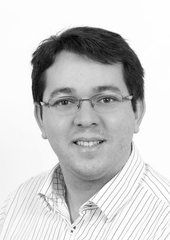
\includegraphics[width=1in,height=1.25in,clip,keepaspectratio]{lucas3por4}}]{Lucas Cordeiro}
received his Ph.D. degree in Computer Science in 2011 from the University of Southampton, UK. Currently, he is a Senior Lecturer in the School of Computer Science at the University of Manchester, UK and leads the Systems and Software Verification laboratory. He is also a collaborator in the Postgraduate Program in Electrical Engineering and Informatics at the Federal University of Amazonas (UFAM), Brazil. Prior to joining the University of Manchester, he worked as a researcher / researcher engineer at Oxford University / Diffblue and as an adjunct professor at UFAM; he also worked for 4 years as a software engineer at Siemens Mobile and CT-PIM. His work focuses on software model checking, automated testing, program synthesis, and embedded \& cyber-physical systems.
\end{IEEEbiography}

% insert where needed to balance the two columns on the last page with
% biographies
%\newpage

%\begin{IEEEbiographynophoto}{Jane Doe}
%Biography text here.
%\end{IEEEbiographynophoto}

% You can push biographies down or up by placing
% a \vfill before or after them. The appropriate
% use of \vfill depends on what kind of text is
% on the last page and whether or not the columns
% are being equalized.

%\vfill

% Can be used to pull up biographies so that the bottom of the last one
% is flush with the other column.
%\enlargethispage{-5in}



% that's all folks
\end{document}


